\documentclass[final]{nuthesis}
\usepackage{amssymb, amsthm, amsmath, amsfonts}
\usepackage{mathrsfs}
\usepackage{hyperref}
\usepackage{graphicx}
\usepackage{lineno}
\usepackage{listings}
\usepackage{float}
\usepackage{multicol}
\usepackage{xr}

\externaldocument{An_IPM_For_Indeterminate_Growth/An_IPM_For_Indeterminate_Growth}
\externaldocument{Spectral_Properties/Spectral_Properties}
\externaldocument{Estimating_the_Spectral_Radius/Estimating_the_Spectral_Radius}
\externaldocument{Simulations_of_a_Density-Dependent_Growth_Model/Simulations_of_a_Density-Dependent_Growth_Model}

\newtheorem{theorem}{Theorem}
\newtheorem{definition}{Definition}
\newtheorem{proposition}{Proposition}
\newtheorem{lemma}{Lemma}
\newtheorem{corollary}{Corollary}
\theoremstyle{definition}
\newtheorem{example}{Example}[section]

\numberwithin{theorem}{section}
\numberwithin{lemma}{section}
\numberwithin{corollary}{section}
\numberwithin{definition}{section}
\numberwithin{equation}{section}

\newcommand{\ms}{\mathscr}
\DeclareMathOperator{\SPAN}{span}
\DeclareMathOperator{\ESSSUP}{ess \, sup}
\DeclareMathOperator{\eig}{eig}

\newcommand{\R}{\mathbb{R}}
\newcommand{\C}{\mathbb{C}}
\newcommand{\N}{\mathbb{N}}
\newcommand{\dd}{\delta}
\newcommand{\ee}{{{\varepsilon}}}

%%% The following commands make the "chi" character look better with subscripts

\makeatletter
\@ifdefinable\@latex@chi{\let\@latex@chi\chi}
\renewcommand*\chi{{\@latex@chi\smash[t]{\mathstrut}}}
\makeatletter

\begin{document}

\frontmatter

\title{Spectral Properties of a Non-Compact Operator in Ecology}
\author{Matt Reichenbach}
\adviser{Professors Richard Rebarber and Brigitte Tenhumberg}
\adviserAbstract{Richard Rebarber and Brigitte Tenhumberg}
\major{Mathematics}
\degreemonth{December}
\degreeyear{2020}
%%
%% For most people the defaults will be correct, so they are commented
%% out. To manually set these, just uncomment and make the needed
%% changes.
%% \college{Your college}
%% \city{Your City}
%%
%% For most people the following can be changed with a class
%% option. To manually set these, just uncomment the following and
%% make the needed changes.
%% \doctype{Thesis or Dissertation}
%% \degree{Your degree}
%% \degreeabbreviation{Your degree abbr.}
%%
%% Now that we know everything we need, we can generate the title page
%% itself.
%%
\maketitle
%%
%% You have a maximum of 350 words for your abstract, which includes
%% your title, name, etc.
%%
%% Required
\begin{abstract}
		Ecologists have used integral projection models (IPMs) to study fish and other animals which continue to grow throughout their lives. Such animals cannot shrink, since they have bony skeletons; a mathematical consequence of this is that the kernel of the integral projection operator $T$ is unbounded, and the operator is not compact. \emph{A priori}, it is unclear whether these IPMs have an asymptotic growth rate $\lambda$, or a stable-stage distribution $\psi$. In the case of a compact operator, these quantities are its spectral radius and the associated eigenvector, respectively. Under biologically reasonable assumptions, we prove that the non-compact operators in these IPMs share important spectral properties with their compact counterparts. Specifically, we show that the operator $T$ has a unique positive eigenvector $\psi$ corresponding to its spectral radius $\lambda$, the spectral radius $\lambda$ is strictly greater than the supremum of all other spectral values, and for any nonnegative initial population $\varphi_0$, there is a $c>0$ such that $T^n\varphi_0/\lambda^n \to c \cdot \psi$. We also show that the zeros of certain functions defined by sums of compact operators can be used to approximate the spectral radius $\lambda$ of the non-compact operator $T$. In the final chapter, we give some simulations showing the long-term behavior of a density-dependent IPM.
\end{abstract}


%% Optional
%% \begin{copyrightpage}
%% \end{copyrightpage}

%% Optional
\begin{dedication}
    I dedicate this thesis to my parents, for always supporting me (no matter what hairbrained thing I decide to do).
\end{dedication}

%%%%%%%%%%%%%%%%%%%
% Acknowledgments
%%%%%%%%%%%%%%%%%%%
\begin{acknowledgments}
	There are many people without whom I never would have been able to write this thesis. First, I want to thank my advisors, Richard Rebarber and Brigitte Tenhumberg. 
	
	Second, I want to thank my family for their constant love and support.
	
	Finally, I give my heartfelt thanks to all of the friends I've made here in Lincoln.
\end{acknowledgments}
%%%%%%%%%%%%%%%%%%%

%%%%%%%%%%%%%%%%%%%
% Grant Information
%%%%%%%%%%%%%%%%%%%
% \begin{grantinfo}
%     % Add any grant info here
% \end{grantinfo}

%%%%%%%%%%%%%%%%%%%
% ToC
%%%%%%%%%%%%%%%%%%%
\tableofcontents

%%%%%%%%%%%%%%%%%%%
% List of Figures
%%%%%%%%%%%%%%%%%%%
\listoffigures
\listoftables

%%%%%%%%%%%%%%%%%%%
% Start of the document
%%%%%%%%%%%%%%%%%%%
\mainmatter

%% Input each chapter as its own file here
\chapter{An Integral Projection Model For Indeterminate Growth}

\section{Integral Projection Models in Ecology} \label{section:ipmsinecology}

In this thesis, we study operators which arise in \emph{integral projection models} (or \emph{IPMs}) describing animal populations in which the individuals exhibit indeterminate growth; that is, when individuals continue to grow throughout their lives. The operators in IPMs are not projections in the mathematical sense of the word; the term \emph{projection} comes from the fact that these models ``project" a current population size and structure into the future. We will exclusively use the term \emph{IPM} hereafter to avoid confusion.

IPMs are discrete-time, stage-structured models introduced in \cite{Easterling1998} and \cite{Ellner2006}; they generalize Leslie matrices (see \cite{Caswell2001}) by allowing for the structure variable to take on values in a continuum. Hence, IPMs are appropriate when vital rates depend on a continuous variable, such as the length or biomass of an individual. The paper \cite{Briggs2010} is a gentle introduction to constructing IPMs, whereas \cite{Ellner2016} is a more detailed overview.

The IPMs we consider in this thesis are given by an integral operator $T:L^1 \to L^1$ where
\[\varphi_{t+1}(y) = (T\varphi_t)(y) := \int_L^U k(y,x) \varphi_t(x) \, dx.\]
Here, $\varphi_{t}(x)$ is the population density in stage $x$ at time $t$, the nonnegative kernel function $k(y,x)$ describes how the distribution of individuals in stage $x$ contributes to the individuals in stage $y$ in the next time step, and $L$ and $U$ are the lower- and upper-limits of the structure variable, respectively. We assume that the kernel function $k(y,x)$ can be decomposed as 
\[k(y, x) = s(x) g(y,x) + b(y)f(x),\]
where $s(x)$ is the survival probability of an individual in stage $x$, $g(y,x)$ gives the probability that a stage $x$ individual grows to a stage $y$ individual in one time step, $b(y)$ is the size distribution of newborns, and $f(x)$ gives the expected number of offspring that an average individual in stage $x$ will produce in one time step. We will refer to $s(x)g(y,x)$ as the \emph{survival and growth} subkernel, and $b(y)f(x)$ as the \emph{fecundity} subkernel. In practice, these functions are usually determined by fitting appropriate curves to population data.

IPMs have found wide use in the biological sciences \cite{Ellner2016}. In the case that the kernel function $k(y,x)$ is continuous and positive on the square $[L, U]^2$, the associated IPM operator $T$ has its spectral radius as an eigenvalue, and the associated eigenvector is nonnegative (among other things) \cite{Ellner2006}. In biological terms, the spectral radius of the operator $T$ is the asymptotic growth rate of the population, which we will denote by $\lambda$, and the associated eigenvector $\psi$ is the stable stage distribution. The eigenvector $\psi$ is important in conservation biology, because by comparing the stable stage distribution with a population distribution in the field, a biologist can determine if the field population has reached the steady state. 

In the case that the kernel function $k(y, x)$ is bounded, $T$ is a compact operator on the relevant function space \cite{Ellner2006}. Compact operators can be uniformly approximated by matrices, which is one reason why an IPM with a compact operator is easier to work with. When a IPM operator is compact, ecologists can estimate the asymptotic growth rate of a population by approximating the infinite-dimensional operator with large matrices. The leading eigenvalues of these large matrices can thus give a good approximation of the asymptotic growth rate of the population, when modeled by an IPM.

The appropriate choice for the structure variable depends on the ecology of the species being modeled, or what data ecologists can collect. Some common examples of structure variables in IPMs are animal biomass, stem diameter of plants, the proportion of tissue infected by a disease, and the length or height of individuals. However, this choice has mathematical consequences: if individuals can decrease in size from one time step to the next, the IPM operator $T$ will be compact; if individuals cannot decrease in size, we prove in Section \ref{section:noncompactness} that $T$ will not be compact. In the former case, the results in \cite{Ellner2006} apply to the operator $T$.

For structure variables that cannot decrease over time, i.e., when the probability of shrinkage is zero, the growth subkernel $g(y, x)$ is unbounded. To get an intuitive idea for why this is the case, suppose that $G$ is the integral operator with kernel $g(y, x)$; this operator models the somatic growth of individuals over one time step. If individuals cannot shrink, and must continue to grow, then applying $G$ repeatedly yields a population dominated by individuals near the maximum body size. Since $g(y, x)$ does not incorporate mortality, the growth subkernel $g(y, x)$ must capture the growth of an increasingly concentrated population. Hence, $g(y, x)$ will be unbounded near the point $(U, U)$, where $U$ is the maximum body size. If the function $g(y, x)$ is unbounded, then the full IPM kernel $k(y, x)$ will be as well. 

In general, it is possible for compact integral operators to have unbounded kernels; if this were the case for an IPM operator $T$, then the results proved in \cite{Ellner2006} would still apply. But in this paper, we will show that assuming individuals do not shrink implies not only that the kernel $k(y, x)$ is unbounded, but also that the associated integral operator is not compact. This means that the results proved in \cite{Ellner2006} do not apply to these populations, thus making it unclear whether IPMs with non-compact operators have an asymptotic growth rate or a stable stage distribution.

Most IPMs in the literature have compact operators. Examples include those which model plant species that can shrink over time in poor growing conditions (\cite{Childs2003, Eager2013, Hegland2010, Jacquemyn2010, Miller2012, Tenhumberg2015, Rees2002}.  Additionally, \cite{Childs2011, Ellner2016, Coulson2011} used the biomass of sheep and wolf individuals as their structure variable, which can also decrease in poor environmental conditions. The paper \cite{Bruno2011} models the proportion of coral covered by a fungal infection, which can decrease over the course of a time step. Alternatively, some papers have used the length of fish and mollusks as structure variables, namely \cite{Aalto2019, Ohlberger2020, Stubberud2019, Vindenes2014} and \cite{Vindenes2015}, presumably because these were the only data available for parameterizing their IPM models. Since length cannot decrease from one time step to the next, their IPM operators are non-compact.

In this thesis, we show that biologically relevant properties, such as the existence of an asymptotic growth rate and a stable stage distribution for the population, still hold for the non-compact IPM operator $T$. This allows ecologists to gain biological insight from IPMs in which individuals cannot shrink between time steps.

\section{Mathematical Motivations} \label{section:mathematicalmotivations}

IPMs are generalizations of matrix population models of the form
\begin{align}
	\vec{n}_{t+1} = A \vec{n}_t, \quad \vec{n}_0 \in \R^n, \label{eqn:system}
\end{align}
where $A$ is a matrix, and $\vec{n}_0$ a population vector, both with non-negative entries. The relevant spectral properties of the matrix $A$ in these models are guaranteed by the Perron-Frobenius Theorem (see \cite{Caswell2001}). Among other things, population matrices have the following three properties:
\begin{enumerate}
	\item \label{pf:radius} the spectral radius $r(A)$ is positive, and is an eigenvalue for $A$. The right and left eigenvectors $\vec{v}$, $\vec{v}^*$ associated to $r(A)$ are the only eigenvectors of $A$ which can be normalized to have all positive entries;
	\item \label{pf:inequality} the operator $A$ has a ``spectral gap", meaning that
	\[\max\{\sigma(A) \setminus \{\lambda\}\} < r(A);\]
	\item \label{pf:limit} for any $\vec{n}_0 \in \R^n$ with nonnegative entries, and $\lambda=r(A)$ the spectral radius of $A$ associated to the right and left eigenvectors $\vec{v}$, $\vec{v}^*$, we have $ \langle \vec{n}_0, \vec{v}^* \rangle > 0$, and 
	\[\lim_{k \to \infty} \frac{A^k \vec{n}_0}{\lambda^k} = \langle \vec{n}_0, \vec{v}^* \rangle \vec{v},\]
	where $\langle \cdot, \cdot \rangle$ denotes the dot product in $\R^n$.
\end{enumerate}

In biological terms, property (\ref{pf:limit}) means that the population has a long-term growth rate of $\lambda = r(A)$, and the vector $\vec{v}$ is known as the \emph{stable stage distribution}. The vector $\vec{v}$ gives the relative proportions of each stage in the long-term population, or in other words, $\vec{v}$ captures the proportions one would expect to see in the population absent any external perturbations.

The results in \cite{Krein1950} show that certain compact operators have property (\ref{pf:radius}), and many authors have since obtained generalizations of this result for wider classes of operators (for example, see the papers \cite{Anselone1974, Bonsall1958, Edmunds1972, Karlin1959, Kras1989, Lubben2009, Marek1967, Marek1970, Raghavan1965}, and \cite{Schaefer1960}). Various authors have also obtained results like (\ref{pf:inequality}) for a wider class of operators (see e.g. Chapter 12 of the book \cite{Kras1989}, and the references cited therein). In an appendix to the the paper \cite{Ellner2006}, the authors showed that certain compact operators arising from IPMs in mathematical ecology satisfy properties (\ref{pf:radius}), (\ref{pf:inequality}), and (\ref{pf:limit}).

In this thesis, we consider a class of operators which come from IPMs recently constructed by mathematical ecologists, but for which the results in \cite{Ellner2006} do not apply. Specifically, the operators we consider are not compact. Out of the papers listed above, \cite{Bonsall1958, Edmunds1972, Karlin1959, Kras1989, Marek1967, Marek1970, Raghavan1965, Sawashima1964, Schaefer1960} considered operators $T:X \to X$ which are not necessarily compact. Instead, the authors impose topological conditions on the space $X$, or specific conditions on the operator $T$, in order to prove their results.  We note that IPMs are \emph{discrete-time} models, but results like (1)-(3) above are known for \emph{continuous-time} models as well; see Chapters 8-10 in the book \cite{Clement1987}. 

For our purposes, the results proved in \cite{Marek1970}, \cite{Sawashima1964}, and \cite{Schaefer1960} will be useful to us in showing that the operators we consider have properties (\ref{pf:radius}) - (\ref{pf:limit}) of the Perron-Frobenius Theorem. Specifically, we will show that the operator $T:L^1 \to L^1$ is not compact, that it is \emph{strictly nonsupporting}, and that its spectral radius $r(T)$ is a pole of the resolvent operator $R(z, T)$. We will prove these facts in Sections \ref{section:noncompactness}, \ref{section:nonsup}, and \ref{section:pole} respectively. In Section \ref{section:mainresults}, we will show that the non-compact operator $T$ has properties (\ref{pf:radius})-(\ref{pf:limit}) above. This means that IPMs with non-compact operators of the form we consider have the theoretical properties one would want in a population model.

\section{Definition of the IPM Operator and its Components} \label{section:operatordef}

For functional analysis concepts and notation, we follow \cite{Conway1994}. All integrals will be with respect to the Lebesgue measure $\mu$, and ``a.e" means ``almost-everywhere" with respect to $\mu$. Let $\Omega := [L,U]$ denote a closed and bounded interval of $\R$. In IPMs, the limits $L$, $U$ will be positive values denoting the lower- and upper- limits for the structure variable, respectively.

We will use the notation $L^1 : = L^1(\Omega)$ to denote the Banach space of integrable real-valued functions with norm
\[||\varphi||_1 := \int_L^U |\varphi(t)| \, dt.\]
The space $L^1$ is the natural space to work in for biological applications, because the norm $||\varphi||_1$ of the nonnegative population vector $\varphi$ gives the total population. We will also make use of the space $L^\infty = L^\infty(\Omega)$, which is the space of Lebesgue-measurable, essentially bounded functions with norm
\[||h||_\infty := \ESSSUP \{|h(t)| \mid t \in \Omega\}.\]

We study integral operators $T:L^1 \to L^1$ whose kernels take the form
\begin{align}
	k(y,x) = s(x) g(y,x) + b(y) f(x). \label{eqn:kernel}
\end{align}
Here, we will assume that the function $s(x)$ is continuous, increasing, and positive on $\Omega$, with 
\[\sup_{x \in \Omega} \{s(x)\} < 1.\]
This means that each individual has a chance of dying during each time step, and the positivity assumption means that any individual has a chance of surviving. We will assume that $b(y)$ is the offspring distribution, bounded almost-everywhere in $\Omega$ and positive almost-everywhere in the set $[L, x_b]$, where we allow (but do not require) that $b(y)$ can be zero for all $y > x_b$. In that case, $x_b$ is the largest size that an individual can attain in one time step after birth.

Additionally, we suppose that there is some $x' \in [L, U)$ such that $f(x)$ is almost-everywhere bounded away from zero for $x \geq x'$. We have been unable to find an IPM in which these assumptions on $f(x)$ are not satisfied, and our results apply just as well when $f(x) > 0$ throughout $\Omega$ (in this case, one can take $x' = L$).

Taken together, these assumptions on $s(x)$, $b(y)$, and $f(x)$ imply the existence of positive numbers, $s_0$, $s_1$, $b_1$, and $f_0$, $f_1$ such that
\begin{align}
	&0 < s_0 \leq s(x) \leq s_1 < 1, \quad \text{for almost every } x \in \Omega, \label{eqn:s(x)bounds} \\
	&0 < b(y) \leq b_1 < \infty, \quad \text{for almost every } y \in \Omega, \label{eqn:b(y)bounds} \\
	&0 < f_0 \leq f(x) \leq f_1 < \infty, \quad \text{for almost every } x \in [x', U] \label{eqn:f(x)bounds}
\end{align}
It will be convenient to assume that $s_1$, $b_1$, $f_1$ are the least such values, and that $s_0$, $f_0$ are the greatest such values.

We assume that $g(y,x)$ is nonnegative on $[L,U)^2$ (note the open right endpoint), and also that for each $x \in [L,U)$,
\begin{align}\int_L^U g(y,x) \, dy = 1. \label{eqn:gyx=1}\end{align}
The assumption (\ref{eqn:gyx=1}) means that $g(y,x)$ is a probability distribution for each fixed $x \in [L, U)$. In biological terms, this means that a size $x$ individual will have size $y \in [L,U)$ in the following time step with probability $g(y, x)$. We will often refer to $g(y,x)$ as the \emph{growth subkernel} of $T$.

Of particular interest to us in this paper are operators with a kernel of the form (\ref{eqn:kernel}) such that
\begin{align}
	g(y,x) = 0, \quad \text{whenever } y < x, \label{eqn:gyx=0}
\end{align} 
and in this case we will say that $g(y,x)$ is ``zero below the diagonal". When the operator $T$ models a stage-structured population such that individuals cannot move to lower stages (for example, when $\Omega$ is a set of possible lengths, and individuals exhibit indeterminate growth), $g(y,x)$ satisfies (\ref{eqn:gyx=0}). Note that we do not require $g(y, x)$ to be continuous, so in particular it may be positive for $y=x$ and still satisfy \eqref{eqn:gyx=0}.

Taken together, assumptions (\ref{eqn:gyx=1}) and (\ref{eqn:gyx=0}) imply that $g(y,x)$ is unbounded in any neighborhood of the point $(U, U) \in \R^2$, which is why we assume $g(y,x)$ is defined on $[L,U)^2$, rather than $[L,U]^2$. 

\begin{example}
	We have included Figure \ref{fig:growth-kernel-plot} below as an example of an unbounded growth kernel from \cite{Vindenes2014}; they include an extra parameter $z$ for temperature, which we set to 10.34, the mean of the time series they consider. The function in Figure \ref{fig:growth-kernel-plot} is given by
	\[g(y, x) = \left\{ \begin{array}{lc} \frac{\rho(y, x)}{\int_x^U \rho(y, x) \, dy}, & y \geq x, \\ 0, & y < x \end{array} \right. ,\]
	where
\begin{align}
	\rho(y, x) &:= \frac{1}{\sqrt{2 \pi}(y - x) v(x)} \exp \left( - \frac{(\ln(y - x) - \mu(x))^2}{2 v(x)} \right), \label{eqn:rhodef}\\
	\mu(x) &:= \log \left( \frac{(m(x)-x)^2}{\sqrt{(m(x) - x)^2 + \sigma(x)^2}}\right), \label{eqn:linearmudef} \\
	v(x) &:= \log \left( 1 + \frac{\sigma(x)^2}{(m(x)-x)^2}\right).	\label{eqn:linearvdef}
\end{align}
	Equation \ref{eqn:rhodef} is the lognormal probability density function for the growth increment $(y - x)$. In equations \eqref{eqn:linearmudef} and \eqref{eqn:linearvdef}, the function $m(x)$ is the ``average expected size" function (which is usually fit to population data), and $\sigma(x)$ is the standard deviation of sizes at size $x$. Also, note that $m(x)$ and $\sigma(x)$ are functions of the size $x$ on a linear scale, hence why the conversions \eqref{eqn:linearmudef} and \eqref{eqn:linearvdef} are necessary.
	\begin{center}
		\begin{figure}
			\centering
			\includegraphics[width=\textwidth]{"Images/Growth Kernel Plot"}
			\caption{The growth kernel $g(y,x)$ for the northern pike IPM} \label{fig:growth-kernel-plot}
		\end{figure}
	\end{center}
	In Figure \ref{fig:growth-kernel-plot}, we left the surface unshaded in the region $y < x$, to indicate that $g(y,x) = 0$ there. This is the way to incorporate the biological assumption that individuals cannot transition to a smaller size; i.e., they cannot ``shrink". Note that the plot becomes unbounded in a neighborhood of the point $(U,U)$, where $U$ is the maximum size.
	
\end{example}

In \cite{Ellner2006}, the IPM kernel is strictly positive and continuous, and hence bounded away from zero in the square $[L, U]^2$. We cannot make this same assumption, because we allow the component functions $g(y,x)$, $b(y)$, and $f(x)$ to possibly be zero in sets of positive measure. Hence, we will need further assumptions to prove similar results to those in \cite{Ellner2006}; we will denote these assumptions by (\textbf{M}), (\textbf{R}), and (\textbf{S}):

\begin{enumerate}
	\item[(\textbf{M})] there is a continuous, strictly increasing function $\eta:[L,U] \to [L,U]$ such that $\eta(U)=U$, $\eta(x)>x$ for all $x \in [L,U)$, and
	\begin{align}
		\int_{\eta(x)}^U g(y,x) \, dy &> 0, \quad \text{for a.e. } x \in \Omega, \label{eqn:M1}\\
		\int_L^{\eta^{-1}(y)} g(y,x) \,dx &> 0, \quad \text{for a.e. } y > \eta(L), \label{eqn:M2}\\
		g(y, x) &> 0, \quad \text{for a.e. } (y, x) \text{ such that } x < y < \eta(x); \label{eqn:M3}
	\end{align}
	\item[(\textbf{R})] there exists an $\ee_1 > 0$ and a closed rectangle $R \subseteq [L, U)^2$ of the form
	\[R := [U - \ee_1, U] \times [t_1, t_2],\]
	such that for  $L \leq t_1 \leq t_2 \leq y$, and $g(y, x) > 0$ almost-everywhere in $R$;
	\item[(\textbf{S})]  there is some $\ee_2 > 0$ such that $s(x) \equiv s_1$ for $x \in [U - \ee_2, U]$.
\end{enumerate} 
When constructing an IPM kernel from data for a specific population, one often fits the average growth function, which gives the mean expected size for an individual of size $x$ to grow to in one time step. Depending on the form of $g(y, x)$, one can usually take take this average growth function to be $\eta$, or a related function like in the example above where $\mu$ satisfies assumption (\textbf{M}). Assumption (\textbf{R}) looks onerous, but if a growth kernel $g(y, x)$ is obtained by fitting positive probability distributions to data, it will satisfy assumption (\textbf{R}). Although (\textbf{S}) is a technical condition we need to prove a result, we believe it is reasonable because the operators in \cite{Ohlberger2020, Stubberud2019, Vindenes2014, Vindenes2015} all satisfy it.

For notational convenience, we will sometimes write $T:L^1 \to L^1$ in terms of its components
\[T = GS + bF,\]
where $G:L^1 \to L^1$ is the integral operator with kernel $g(y,x)$, $S:L^1 \to L^1$ is multiplication by $s(x)$, $F:L^1 \to \R$ is the fecundity functional defined by
\[\varphi \mapsto \int_L^U f(t) \varphi(t) \, dt,\]
and $b$ is the offspring distrubition. We will call $G$ the growth operator, the composition $GS$ as the ``growth and survival" operator, and $bF$ the ``fecundity" operator.

\section{Mathematical Preliminaries} \label{section:mathprelims}

Given a Banach space $X$, we denote the space of continuous linear functionals on $X$ as $X^*$; the space $X^*$ is known as the Banach dual space of $X$. In this paper, we will only consider the case where $X=L^1$, in which case $X^* = L^\infty$, and the functionals are represented by some $h \in L^\infty$ acting by integration on elements in $L^1$. We will use the inner-product notation $\langle \varphi, h \rangle$ to denote this action; that is, for $\varphi \in L^1$ and $h \in L^\infty$, we define
\begin{align}
	\langle \varphi, h \rangle := \int_L^U \varphi(t) \, h(t) \, dt. \label{eqn:functional}
\end{align}
We will sometimes abuse terminology by referring to the element $``h"$ as a functional, but it should be clear we mean it represents a functional given by \eqref{eqn:functional}.

Given a linear operator $T:X \to Y$ between normed vector spaces $X$ and $Y$, we denote the \emph{operator norm} of $T$ to be the quantity
\[||T|| := \sup \{ ||T\varphi||_Y \mid ||\varphi||_X = 1\},\]
where the subscripts denote which space the norm is taken in. If this operator norm is finite, we say that $T$ is a bounded operator. It is straightforward to show that the integral operator $T:L^1 \to L^1$, with kernel $k(y, x)$ satisfying \eqref{eqn:kernel} - \eqref{eqn:gyx=1}, is bounded.

The Banach adjoint of $T$, denoted $T^*:X^* \to X^*$, is the unique operator such that
\[\langle T \varphi, h \rangle = \langle \varphi, T^*h \rangle,\]
for all $x \in X$ and $h \in X^*$.

For a linear operator $T:X \to X$, with $X$ a vector space over $\C$, the \emph{spectrum} of $T$ is the set
\[\sigma(T) := \{z \in \C \mid z I- T \text{ is not boundedly invertible}\}.\]
Here, $I$ is the identity operator. Additionally, we denote the \emph{spectral radius} of the operator $T$ by $r(T)$, where
\[r(T) := \sup \{ |z| \mid z \in \sigma(T)\}.\]
The \emph{peripheral spectrum} $\sigma_p(T)$ are those $z \in \sigma(T)$ such that $|z| = r(T)$. 

Another subset of $\sigma(T)$ which will be useful to us is known as the \emph{essential spectrum}; we will denote this subset by $\sigma_e(T)$. There many definitions of the essential spectrum in the literature, but we use the one given in \cite{Browder1961} and \cite{Edmunds1972}:

\begin{definition}
	The \emph{essential spectrum} $\sigma_e(T)$ of an operator $T$ is the collection of complex numbers $z \in \sigma(T)$ such that at least one of the following conditions holds:
	\begin{enumerate}
		\item the range of $(z I - T)$ is not closed;
		\item $z$ is a limit point of $\sigma(T)$;
		\item $\cup_{n=1}^\infty \ker (z I- T)^n$ is infinite-dimensional,
	\end{enumerate}
	where $\ker(\cdot)$ denotes the kernel of its argument.
\end{definition}

We also make use of the \emph{essential spectral radius} of the operator $T$, which we denote $r_e(T)$, and which is defined analogously to the ordinary spectral radius:
\[r_e(T) := \sup \{ |z| \mid z \in \sigma_e(T)\}.\]
For the other common definitions of the essential spectrum, each has the same essential spectral radius, a fact proved in \cite{Edmunds1987}.

Note that the operators in IPMs are naturally operators on a real vector space; in order to talk about the spectrum of an operator $T:X \to X$, with $X$ a vector space over $\R$, we define the \emph{complexifications} of $T$ and $X$, denoted $T_c$ and $X_c$, where
\begin{align}
	X_c := X \oplus i X \label{eqn:complexifyxpace},
\end{align}
and $T_c: X_c \to X_c$ is the linear operator such that
\begin{align}
	T_c(\varphi_1 + i \varphi_2) := T(\varphi_1) + i T(\varphi_2). \label{eqn:complexifyT}
\end{align}
When we refer to ``the spectrum of $T$", where $T$ is an operator on a real vector space, we actually mean the spectrum of its complexification $T_c$. One can show that $X_c$ is a Banach space over $\C$, with addition and scalar multiplication defined in the natural way, and with the norm $|| \cdot ||_c$ defined by
\[||\varphi_1 + i \varphi_2||_c := \frac{1}{\sqrt 2} \cdot \sup_{0 \leq \theta < 2\pi} (||\cos( \theta ) \varphi_1 - \sin( \theta ) \varphi_2|| + ||\sin( \theta ) \varphi_1 + \cos( \theta ) \varphi_2 ||)\]
The complexification $T_c$ is linear and bounded if and only if $T$ is also linear and bounded. Additionally, the norms of $T$ and $T_c$ coincide:
\begin{align}
	||T|| = ||T_c||_c. \label{eqn:equalnorms}
\end{align}
For more information concerning complexifications of real vector spaces and operators, see \cite{Edmunds1972}. 

To compute spectral radii, we will make use of Gelfand's formula, which is the statement that
\begin{align}
	r(T) = \lim_{n \to \infty} ||T||^{1/n}. \label{eqn:gelfand}
\end{align}
The \emph{resolvent} of $T$ is the function $R(z, T):= (zI - T)^{-1}$, which is well-defined in the \emph{resolvent set} $\rho(T):= \C \setminus \sigma(T)$. It turns out that $R(z, T)$ is a holomorphic function in $\rho(T)$, and in the case that $|z| > r(T)$, we can write $R(z, T)$ as a so-called \emph{Neumann series} given by
\begin{align}
	R(z, T) &= \sum_{k = 0}^\infty \frac{T^k}{z^{k+1}}. \label{eqn:neumannseries}
\end{align}	

In order to study the essential spectrum $\sigma_e(T)$, we will make use of the \emph{ball measure of non-compactness}, or \emph{ball MNC} for short. Some authors also use the term \emph{Hausdorff MNC}. We follow the definitions, terminology, and results in \cite{Akhmerov1992}:

\begin{definition} \label{th:betadef}
	The \emph{ball measure of non-compactness} of a subset $V$ of the vector space $X$, denoted $\beta(V)$, is given by
	\[\beta(V):= \inf\{ r>0 \mid V \text{ can be covered by finitely many balls of radius } r \}.\]
	Clearly $0 \leq \beta(V) \leq \infty$; other properties of $\beta(\cdot)$ which will be useful to us are:
	\begin{enumerate}
		\item $\beta(V) = 0$ if and only if $V$ is pre-compact (that is, if and only if the closure of $V$ is compact);
		\item For the set
		\[V + W := \{v + w \mid v \in V, w \in W\},\]
		we have
		\[\beta(V+W) \leq \beta(V) + \beta(W)\]
		for all $V$, $W \subseteq X$;
		\item $V_1 \subseteq V_2$ implies that $\beta(V_1) \leq \beta(V_2)$;
		\item $\beta(\lambda V) = |\lambda| \, \beta(V)$ for each $\lambda \in \C$;
		\item For any point $x_0 \in X$, we have $\beta(V+x_0) = \beta(V)$.
	\end{enumerate}
\end{definition}
For further useful properties that $\beta$ satisfies, see \cite{Akhmerov1992}. There are other commonly used MNC's, but the ball-MNC $\beta$ is especially useful for us because there is a formula for $\beta(V)$ when  $V \subseteq L^p(\R)$, $1 \leq p \leq \infty$. Let $X$ be one of these spaces, and $V \subseteq X$ any subset. Then we have that
\begin{align}
	\beta(V) = \frac 12 \lim_{\delta \to 0} \sup_{\varphi \in V} \sup_{0<\tau \leq \delta} ||\varphi - \varphi_\tau||_X \label{eqn:betaformula}
\end{align}
where $\varphi_\tau(t) := \varphi(t + \tau)$.

We note that the domain of the functions we consider is $\Omega = [L,U]$, but we can apply (\ref{eqn:betaformula}) by extending their domain to all of $\R$ by setting $\varphi(x) = 0$ for $x$ outside $\Omega$, for every $\varphi \in L^1(\Omega)$.

There is a formula for $r_e(T)$, first given in \cite{Nussbaum1970}, which makes use of the ball-MNC $\beta$. Letting $\ms U \subseteq X$ denote the unit ball in the space $X$, and writing $\beta(T) := \beta(T(\ms U))$, we have that
\begin{align}
	r_e(T) = \lim_{n \to \infty} \beta(T^n)^{1/n} \label{eqn:esr}
\end{align}
Note the similarity between this formula for the essential spectral radius, and Gelfand's formula \eqref{eqn:gelfand} for the ordinary spectral radius. Using the formulas (\ref{eqn:betaformula}) and (\ref{eqn:esr}) together, we will be able to compute the essential spectral radius of the non-compact operator $T:L^1 \to L^1$ in Section {\ref{section:pole}.

The operators we study in this paper are examples of \emph{positive} operators, which means that they are invariant on a cone $K$ in a Banach space $X$. We follow the book \cite{Kras1989} for definitions and theorems regarding cones.
	\begin{definition}
		A closed convex set $K$ of the real Banach space $X$ is called a \emph{cone} if the following conditions hold:
		\begin{enumerate}
			\item for any $x \in K$ and $a \geq 0$, the element $ax$ is in $K$,
			\item for any pair $x$, $y \in K$, the element $x +y$ is in $K$, and 
			\item $K \cap -K = \{0\}$.
		\end{enumerate}
	\end{definition}
	
	Defined in this way, we get a partial ordering on the cone $K$: for two elements $x$, $y \in K$, we say that $x \leq y$ if and only if $y-x \in K$. 
	
	It is straightforward to check that the collections of nonnegative a.e. functions in $L^1$ and $L^\infty$ are cones; we refer to these as the \emph{standard cones} in their respective spaces.
	
	Given a cone $K$, we will also make use of its dual cone:
	
	\begin{definition}
		Suppose that $X$ is a Banach space with cone $K$, and let $X^*$ be the Banach dual space of $X$. The \emph{dual cone} of $K$, denoted $K^* \subseteq X^*$, is the collection of all continuous linear functionals $h$ such that $h(x) \geq 0$, for all $x \in K$.
	\end{definition}
	
	It is a straightforward exercise to show that if $K$ is the standard cone in $L^1$, its dual cone $K^*$ is the standard cone in $L^\infty$. For the next definition, we use the notation
	\[K-K := \{x-y \mid x, y \in K\}.\]
	
	\begin{definition}
		An operator $T:X \to X$, (possibly nonlinear), with $X$ a real Banach space,  is called \emph{positive} with respect to a cone $K \subseteq X$ if $T(K) \subseteq K$.
	\end{definition}
	This definition yields a partial order on the set of positive operators: if $T_1$, $T_2$ are positive operators, we say that $T_1 \leq T_2$ if $T_2 - T_1$ is a positive operator.
	
	We will sometimes call an operator simply ``positive", and drop references to the particular cone $K$, as we are only concerned with the standard cones $K \subseteq L^1$ and $K^* \subseteq L^\infty$. Hereafter, when we write $K$ and $K^*$, we mean the standard cones in $L^1$, $L^\infty$ respectively.
	
	\begin{example}
		Supposing it is well-defined, the integral operator $T:L^1 \to L^1$ of the form
		\[(T\varphi)(y) := \int_L^U k(y,x) \varphi(x) \, dx\]
		is an example of a positive operator with the respect to $K$, whenever $k(y,x) \geq 0$ almost-everywhere. Additionally, the Banach dual $T^*:L^\infty \to L^\infty$ is also a positive operator in that it maps $K^*$ into $K^*$, and is given by
		\[(T^* \varphi^*)(x) = \int_L^U k(y,x) \varphi^*(y) \, dy.\]
		That is, the Banach adjoint of an integral operator is obtained by ``transposing" the kernel function, i.e., by integrating with respect to $y$ instead of $x$.
	\end{example}
	
	In Section \ref{section:nonsup}, we will show that the IPM operator in this paper is \emph{strictly nonsupporting}, which is a concept introduced in \cite{Sawashima1964}, and further elaborated in \cite{Marek1970, Niiro1966a} and \cite{Niiro1966b}. We follow the terminology of \cite{Marek1970} on this topic:
	
	\begin{definition} \label{def:nonsup}
		Suppose $T$ is a positive operator with respect to the cone $K$, and suppose that $\varphi \in K$, $\varphi^* \in K^*$ are both nonzero.
		\begin{enumerate}
			\item $T$ is called \emph{nonsupporting} if for every pair $\varphi$, $\varphi^*$ there is a positive integer $p = p(\varphi, \varphi^*)$ such that $\langle T^n \varphi, \varphi^* \rangle >0$ for every $n \geq p$.
			\item $T$ is called \emph{strictly nonsupporting} if for every pair $\varphi$, $\varphi^*$ there is a positive integer $p=p(\varphi)$ such that $\langle T^n \varphi, \varphi^* \rangle > 0$ for every $n \geq p$.
		\end{enumerate}
	\end{definition}
	Note that if $T$ is strictly nonsupporting, it is also nonsupporting. We will also make use of the following concepts in proving our main results:
	
	\begin{definition}
		Given a cone $K$, an element $\varphi \in K$ is called \emph{quasi-interior} if $\langle \varphi, \varphi^* \rangle > 0$ for all nonzero $\varphi^* \in K^*$.
	\end{definition}
	
	\begin{definition}
		Given a cone $K$, an element $\varphi^* \in K^*$ is called \emph{strictly positive} if $\langle \varphi, \varphi^* \rangle > 0$ for all nonzero $\varphi \in K$.
	\end{definition}
\chapter{Spectral Properties of the IPM Operator $T$}

\section{General Results} \label{section:general}

In this section, we will prove some fundamental facts about the operator $T:L^1 \to L^1$ which will be useful in demonstrating many of the results that follow. In particular, at the end of Section \ref{section:noncompactness} we will prove that no power $T^k$ is weakly compact (and in particular not compact) under the assumption (\ref{eqn:gyx=0}). This indicates that we will not be able to use the Krein-Rutman theorem, or its generalizations given in \cite{Kras1989}, to obtain results about the spectral properties of $T$.

\begin{lemma} \label{th:norm=1}
	Let $G:L^1 \to L^1$ be the growth operator, and consider the standard cone $K \subseteq L^1$. Then for any $\varphi \in K$, we have that $||G \varphi||_1 = ||\varphi||_1$.
\end{lemma}

\begin{proof}
	This is a quick application of Fubini-Tonell:
	\begin{align*}
		||G\varphi||_1 &= \int_L^U \int_L^U g(y,x) \varphi(x) \, dx = \int_L^U \varphi(x) \underbrace{\int_L^U g(y,x) \, dx}_{=1, \, \text{a.e. } x} \, dy = ||\varphi||_1,
	\end{align*}
	where the last equality comes from the fact that $\varphi \geq 0$.
\end{proof}

\begin{corollary} \label{th:corollarytonorm=1}
	For each $k \geq 1$ and $\varphi \in K \subseteq L^1$, we have $||G^k \varphi||_1 = ||\varphi||_1$.
\end{corollary}

We mentioned earlier that the kernel function $g(y,x)$, when zero below the diagonal, models the growth of individuals who cannot shrink; we make this intuition rigorous in the next lemma:

\begin{lemma} \label{th:giszero}
	Suppose that $\varphi \in K \subseteq L^1$ is such that for some $a \in [L,U)$, $\varphi(x) = 0$ whenever $x < a$. Then $(G\varphi)(y) =0$ whenever $y < a$ as well.
\end{lemma}

\begin{proof}
	Take some $\varphi \in K$ satisfying the properties above. Fixing an arbitrary $y<a$, we have that
	\begin{align*}
		(G\varphi)(y) &= \int_L^U g(y,x) \varphi(x) \, dx = \int_a^U g(y,x) \varphi(x) \, dx
	\end{align*}
	since $\varphi(x) = 0$ for $x < a$. Because $y<a$ and $g(y,x) = 0$ whenever $y<x$, we conclude that the second integral above is equal to zero. Since the choice of $y<a$ was arbitrary, we have that $(G\varphi)(y) = 0$ for any $y<a$.
	
\end{proof}

With this result, we immediately obtain the corollary

\begin{corollary} \label{th:corollarytogiszero}
	Suppose $\varphi \in K$ and $a \in [L,U)$ are as in Lemma \ref{th:giszero}. For any $k \geq 1$, we have $(G^k \varphi)(y) = 0$ whenever $y < a$ as well.
\end{corollary}

\begin{lemma} \label{th:etalimit}
	Let $\eta(x)$ be the continuous and increasing function described in \textbf{(M)}. For any $x \in [L,U]$, we have that $\eta^n(x) \to U$ as $n \to \infty$, where
	\[\eta^n(x) := \eta(\eta^{n-1}(x)), \quad \text{and} \quad \eta^0(x) := x.\]
\end{lemma}

\begin{proof}
	The result is immediate for $x = U$, so suppose that $L \leq x <U$. Since $\eta$ is strictly increasing, we have that
	\[x < \eta(x) < \eta^2(x) < \cdots \eta^n(x) < \cdots \leq U\]
	for every $n$. The sequence $\{\eta^n(x)\}$ is increasing and bounded above by $U$, so it must have some limit $M$. We claim that $M = U$; to see this, suppose otherwise that $M < U$. Since $\eta$ is continuous, we have that
	\[M = \lim_{n \to \infty} \eta^n(x) = \eta \left( \lim_{n \to \infty} \eta^{n-1}(x) \right) = \eta(M),\]
	but this contradicts the assumption that $\eta(x) > x$ for all $x < U$. Therefore, we conclude that $\eta^n(x) \to U$ for each $x<U$.
	
\end{proof}

It will be useful to define the truncated growth subkernel $g_0(y,x)$, where
\[g_0(y,x):= \left\{
\begin{array}{lc}
g(y,x), & x \in [L,U), y \geq \eta(x) \\
0, & \text{else}
\end{array}
\right.,
\]
Also, define $G_0:L^1 \to L^1$ to be the integral operator with kernel $g_0(y,x)$. We immediately have that $G_0 \leq G$.

\begin{lemma} \label{th:g0phinotzero}
	For any $\varphi \in K \setminus \{0\}$, the function $G_0 \varphi $ is not the zero-function.
\end{lemma}

\begin{proof}
	We prove the contrapositive, so suppose that $G_0 \varphi = 0$, for some $\varphi \in K$. Then
	\begin{align*}
		0 &= ||G_0 \varphi||_1 \\
		&=\int_L^U \int_L^U g_0(y,x) \varphi(x) \, dx \, dy \\
		&=\int_L^U \varphi(x) \int_L^U g_0(y,x) \, dy \, dx \\
		&=\int_L^U \varphi(x) \int_{\eta(x)}^U g(y,x) \, dy \, dx
	\end{align*}
	which implies that $\varphi \equiv 0$ a.e., since we have assumed that $\int_{\eta(x)}^U g(y,x) \, dy >0$ for a.e. $x \in [L,U)$.
	
\end{proof}

\begin{corollary}
	For any $k \geq 1$, $G_0^k \varphi$ is not the zero function.
\end{corollary}

\begin{lemma} \label{th:growingbig}
	Suppose that $||\varphi||_1 >0$. Then for every $n \in \N$,
	\[\int_{\eta^n(L)}^U (G_0^n\varphi)(y) \, dy >0.\]
\end{lemma}

\begin{proof}
	We proceed by induction. By Lemma \ref{th:g0phinotzero}, we know that $G_0 \varphi$ is nonzero, so $||G_0 \varphi||_1 >0$. By definition of the kernel $g_0$, we have that $g_0(y,x) \equiv 0$ for $x \in [L,U)$ and $y<\eta(L)$, and thus we have
	\[0 < \int_L^U (G_0 \varphi)(y) \, dy = \int_{\eta(L)}^U (G_0 \varphi)(y) \, dy,\]
	so the base-case holds.
	
	Next, suppose that
	\[\int_{\eta^k(L)}^U (G_0^k \varphi)(y) \, dy >0\]
	for some $k$. Then, for the sake of a contradiction, suppose that
	\begin{align}
		0 &= \int_{\eta^{k+1}(L)}^U (G_0^{k+1}\varphi)(y) \, dy \notag \\
		&= \int_{\eta^{n+1}(L)}^U \int_L^U g_0(y,x) (G_0^k \varphi)(x) \, dx \, dy \notag \\
		&=\int_L^U (G_0^k \varphi)(x) \left( \int_{\eta^{n+1}(L)}^U g_0(y,x) \, dy \right) \, dx \label{eqn:etaintegral}
	\end{align}
	Assumption (\textbf M) implies that $\int_{\eta(x)}^U g_0(y,x) \ dy > 0$ for a.e $x \in [L,U)$. This implies that 
	\[0< \int_{\eta^{n+1}(L)}^U g_0(y,x) \, dy = \int_{\eta(\eta^n(L))}^U g_0(y,x) \, dy\]
	for a.e. $x$ in the interval $(\eta^n(L), U)$. Comparison of this with (\ref{eqn:etaintegral}) yields that $G_0^k \varphi = 0$ on the interval $(\eta^n(L),U)$, but this contradicts the induction hypothesis. Therefore,
	\[0< \int_{\eta^n(L)}^U (G_0^n \varphi)(y) dy\]
	for every $n \in \N$.
	
\end{proof}

\begin{corollary} \label{th:cortogrowingbig}
	For any nonzero $\varphi \in K$ and $\ee > 0$, there is an $N \in \N$ such that for $n \geq N$, $G^n\varphi$ is positive on a subset of positive measure in the interval $[U - \ee, U]$.
\end{corollary}

\begin{proof}
	Fix $\ee > 0$, and let $N \in \N$ be the integer guaranteed by Lemma \ref{th:etalimit} such that $\eta^n(L) > U - \ee$ for every $n \geq N$. Applying the result of Lemma \ref{th:growingbig}, we have
	\[\int_{U - \ee}^U (G^n \varphi)(y) \, dy \geq \int_{\eta^n(L)}^U (G^n \varphi)(y) \, dy \geq \int_{\eta^n(L)}^U (G_0^n \varphi)(y) \, dy > 0.\]
	Therefore, $G^n\varphi>0$ on a subset of positive measure in the interval $[U - \ee, U]$ for any $n \geq N$. 
\end{proof}

\section{Each Operator $T^k$ is Not Compact} \label{section:noncompactness}

We now  move on to showing that all powers of the operator $T$, with growth kernel $g(y, x)$ zero below the diagonal, fail to be compact. This is in contrast to the case with a bounded kernel considered in \cite{Ellner2006}. In fact, we will prove a stronger statement: every power $T^k$ fails to be weakly compact. The main result of this section is:

\begin{theorem} \label{th:notweaklycompact}
	For the integral operator $T:L^1 \to L^1$ with kernel given by (\ref{eqn:kernel}) and with $g(y,x)$ zero below the diagonal, the operator $T^k$ is not weakly compact for any $k \geq 1$.
\end{theorem}

\begin{corollary} \label{th:corollarytonotweaklycompact}
	The operator $T^k:L^1 \to L^1$ is not compact for any $k \geq 1$.
\end{corollary}

To prove Theorem \ref{th:notweaklycompact}, we use the fact that weak compactness and weak sequential compactness are equivalent in Banach spaces. This is known as the Eberlein-\v{S}mulian theorem, and is Theorem V.6.1 in \cite{Dunford1958}:

\begin{theorem}[Eberlein-\v{S}mulian] \label{th:eberlein}
	Let $X$ be a Banach space. Then the following are equivalent:
	\begin{enumerate}
		\item $X$ is weakly compact,
		\item $X$ is weakly sequentially compact, and
		\item $X$ is weakly limit-point compact.
	\end{enumerate}
\end{theorem}

We will use the following characterization of weakly sequentially compact sets in $L^1$, which is Theorem IV.8.11 in \cite{Dunford1958}:

\begin{theorem} \label{th:L1weakseq}
	If the family $\ms F \subseteq L^1(S, \sigma, \mu)$ is weakly sequentially compact, then
	\begin{align}
		\lim_{\mu(E) \to 0} \int_E h(s) \, d\mu =0 \label{eqn:weakseq}
	\end{align}
	uniformly for $h \in \ms F$. If $\mu(S) < \infty$, then this condition is sufficient for $\ms F$ to be weakly sequentially compact.
\end{theorem}

For our purposes, the set $S$ is the closed and bounded interval $\Omega = [L,U] \subseteq \R$, which has finite Lebesgue measure; hence, condition (\ref{eqn:weakseq}) is necessary and sufficient to determine weakly sequentially compact collections of $L^1(\Omega)$.

We now have all the ingredients needed to prove the main theorem of this section:

\begin{proof}[Proof of Theorem \ref{th:notweaklycompact}]
	Let $\ms  U \subseteq L^1$ be the closed unit ball. Fix $k \geq 1$, and define $\ms F:=T^k(\ms U) \subseteq L^1$. We note that (\ref{eqn:weakseq}) holds for any fixed $h \in \ms F$; however, we will show that this limit is not uniform on $\ms F$. To this end, put $\dd_n:= \frac 1n (U-L)$ for each $n$, and define $E_n:=[U-\dd_n,U]$; then $\mu(E_n) \to 0$.
	
	Further, define the functions
	\[h_n:= \frac{1}{\dd_n} \cdot \chi_{E_n}(x)\]
	for each $n \geq 1$, where $\chi_{E_n}$ is the characteristic function on $E_n$. Note that
	\[||h_n||_1 = \frac{1}{\dd_n} \int_L^U \chi_{E_n}(x) \, dx = \frac{1}{\dd_n} \int_{U-\dd_n}^U dx = \frac{1}{\dd_n} \cdot \dd_n = 1,\]
	for each $n$. Hence, each $h_n \in \ms U$ and thus $T^kh_n \in \ms F$. Also, Corollary \ref{th:corollarytonorm=1} implies that $||G^k h_n||_1 = 1$, for each $n$.
	
	By assumption on $s(x)$, there is an $s_0$ such that $0 < s_0 \leq s(x)$ for all $x \in [L,U]$. We thus have the lower bound
	\begin{align*}
		\int_{E_n} (T^k h_n)(y) \, dy &\geq s_0^k \int_{E_n} (G^k h_n)(y) \, dy = s_0 ^k \cdot ||G^k h_n||_1 = s_0^k > 0.
	\end{align*}
	This implies that the limit (\ref{eqn:weakseq}) is not uniform on the set $\ms F$. The contrapositive of Theorem \ref{th:L1weakseq} gives that the collection $\ms F$ is not weakly sequentially compact, and the contrapositive of Eberlein-\v{S}mulian implies that that $\ms F$ is not weakly compact. Therefore, $T^k$ fails to be a weakly compact operator for any $k$, since the choice of $k$ was arbitrary.
	
\end{proof}

We note here that the growth operator $G$ is what makes $T^k$ non-compact. By a similar argument as in the previous proof, one can show that the limit (\ref{eqn:weakseq}) is not uniform on the set $G^k(\ms U)$ for any $k \geq 1$.

Theorem \ref{th:notweaklycompact} and its corollary shows that neither the Krein-Rutman theorem, nor its most direct generalization (see Theorem 9.4 in the book \cite{Kras1989}) guarantee that $T:L^1 \to L^1$ has a positive eigenvector corresponding to its spectral radius. 

However, all is not lost: the operator $T$ does have an eigenvector corresponding to its spectral radius, which we prove in Section \ref{section:mainresults}. Before we will be able to do that, we will need to show that $T$ is strictly nonsupporting, and that $\lambda = r(T)$ is a pole of the resolvent $R(z, T)$.

\section{The Operator $T$ is Strictly Nonsupporting} \label{section:nonsup}

Our goal in this section will be to prove that the IPM operator $T$ is \emph{strictly nonsupporting} (see Definition \ref{def:nonsup}). 

We will be able to prove something stronger: for the IPM operator $T$, the integer $p$ in Definition \ref{def:nonsup} will actually be independent of the choice of the nonzero $\varphi \in K$. Also, since we only consider the case when $X = L^1$, showing that $T^n\varphi >0$ almost-everywhere will be sufficient to showing that $T$ is strictly nonsupporting. Hence, the main theorem of this section is:

\begin{theorem} \label{th:nonsup}
	Suppose that the operator $T = GS + bF$ satisfies the assumptions (\textbf{M}) and (\textbf{R}). Then there is a $p \in \N$ such that for every nonzero $\varphi \in K \subseteq L^1$ and $n \geq p$, the element $T^n \varphi$ is positive almost everywhere in $\Omega$.
\end{theorem}
From this, we get the quick corollary:
\begin{corollary} \label{th:cortononsup}
	The operator $T$ is strictly nonsupporting.
\end{corollary}

\begin{proof}[Proof of Corollary \ref{th:cortononsup}]
	Let $p \in \N$ denote the integer guaranteed by Theorem \ref{th:nonsup}, and take any nonzero elements $\varphi \in K$, $\varphi^* \in K^*$. Then $\varphi^*$ acts on elements of $L^1$ by integration, and also $\int_L^U \varphi^*(t) \, dt > 0$, since $\varphi^*$ is nonzero. Fix some $n \geq p$, then we have
	\begin{align*}
		\langle T^n \varphi, \varphi^* \rangle &= \int_L^U (T^n \varphi)(t)\varphi^*(t) \, dt > 0;
	\end{align*}
	since $T^n\varphi$ is positive almost-everywhere, and $\varphi$ is positive on a set of positive measure. Therefore, $T$ is strictly nonsupporting since the nonzero functions $\varphi$, $\varphi^*$ were arbitrary, and so was the choice of $n \geq p$. 
\end{proof}

To prove Theorem \ref{th:nonsup}, we will first give some lemmas:

\begin{lemma}
	Suppose $\varphi(x)>0$ almost-everywhere in $[L, \hat x]$. Then $(G\varphi)(y) > 0$ for almost-every $y \in [L, \eta(\hat x)]$.
\end{lemma}

\begin{proof}
	Since we only need to prove the statement for a.e. $y \in [L, \eta(\hat x)]$, we can assume without loss of generality that $y \in [L, \eta(\hat x)]$ satisfies the inequalities \eqref{eqn:M2} - \eqref{eqn:M3}.
	
	First, suppose that $y \in (L, \eta(\hat x))$; in this case, assumption \eqref{eqn:M3} implies that $g(y, x) >0$ for $(y, x) \in E:=\{y\} \times [L, \hat x]$. Thus, $g(y, x) \varphi(x)>0$ on $E$ as well, so
	\[(G\varphi)(y) = \int_L^U g(y, x) \varphi(x) dx \geq \int_L^{\hat x} g(y, x) \varphi(x) \, dx >0, \]
	as claimed.
	
	Next, suppose that $y \in [\eta(L), \eta(\hat x)]$; in this case, assumption \eqref{eqn:M2} says that
	\[\int_L^{\eta^{-1}(y)} g(y, x) \, dx >0.\]
	This implies that $g(y, x) >0$ on some subset of positive measure contained in $\{y\} \times [L, \eta^{-1}(y)]$. Note also that $\eta^{-1}(y) < \hat x$ since $\eta$ is strictly increasing, so $\varphi(x) >0$ for a.e. $x \in [L, \eta^{-1}(y)]$. Then we have
	\[(G\varphi)(y) = \int_L^U g(y, x) \varphi(x) \, dx \geq \int_L^{\eta^{-1}(y)} g(y, x) \varphi(x) \, dx > 0,\]
	as claimed.
	
\end{proof}

From this, we get the corollary:

\begin{corollary} \label{th:inductivegrowth}
	If $\varphi(x) > 0$ on $[L, \hat x]$, with $\hat x$ as in the above lemma, then $G^k \varphi > 0$ almost-everywhere on $[L, \eta^k(\hat x)]$.
\end{corollary}
The proof of this is immediate, but we also get:
\begin{corollary} \label{th:growth}
	Suppose $\varphi(x) > 0$ almost-everywhere on $[L, \hat x]$. Then for any $\hat y \in [L, U)$, there is an $N \in \N$ such that $G^n \varphi$ is positive almost-everywhere on $[L, \hat y]$ for all $n \geq N$.
\end{corollary}

\begin{proof}
	Fix $\hat y \in (L, U)$. From Lemma \ref{th:etalimit}, we know that $\eta^n(x) \to U$ for any $x \in [L, U]$. Thus, there is an $N = N(\hat x)$ such that $\eta^n(\hat x) > \hat y$ for all $n \geq N$. Since $\eta(\hat x) > \hat x$ and $\eta$ is assumed to be strictly increasing, we have that 
	\[[L, \hat y] \subseteq [L, \eta^N(\hat x)] \subseteq [L, \eta^n(\hat x)],\]
	for all $n \geq N$. Corollary \ref{th:inductivegrowth} says that $G^n \varphi > 0$ almost-everywhere on $[L, \eta^n(\hat x)]$, so we conclude that $G^n \varphi > 0$ almost-everywhere on $[L, \hat y]$ as well, for all $n \geq N$. 
\end{proof}

Note that both Corollaries \ref{th:inductivegrowth} and \ref{th:growth} are still true when applied to the operator $GS$ in place of $G$, since $s(x)$ is positive almost-everywhere. With these facts, we can now prove the main theorem of this section:

\begin{proof}[Proof of Theorem \ref{th:nonsup}]
	Fix some nonzero $\varphi_0 \in K$; then there is an $x_0<U$ such that $\varphi_0(x)>0$ on a subset of positive measure in $[L, x_0]$. Corollary \ref{th:cortogrowingbig} implies that there is some $N_0 \in \N$ such that for $n \geq N_0$, $G^n\varphi_0>0$ on a subset of positive measure in $[x', U]$, where $x'$ is the ``size of maturity" from assumption (\ref{eqn:f(x)bounds}). In particular, we have that $F((GS)^{N_0} \varphi_0) > 0$, so 
	\[\varphi_1 = (T^{N_0 + 1} \varphi_0)(x) \geq b(x) F((GS)^{N_0} \varphi_0) > 0\]
	for almost every $x \in [L, x_b]$, where $x_b$ is the maximum offspring size given in assumption (\ref{eqn:b(y)bounds}).
	
	Next, choose some $y$ with $U - \ee_1 < y < U$, where $\ee_1 > 0$ is the value from assumption (\textbf{R}). Using Lemma \ref{th:etalimit}, choose $N_1 \in \N$ such that $\eta^n(x_b) > y$ for each $n \geq N_1$. Then we have two cases to consider:
	
	\emph{Case 1:} Suppose $x \in [L, U-\ee_1]$. Then Corollary \ref{th:inductivegrowth} implies that
	\[(T^n \varphi_1)(x) \geq ((GS)^n \varphi_1)(x) > 0,\]
	except possibly on a set of measure zero.
	
	\emph{Case 2:} Suppose $x \in (U - \ee_1, U]$. Note that $(GS)^{n - 1}\varphi_1$ is positive almost everywhere on $[L, y]$ by the choice of $N_1$; then for $n \geq N_1 + 1$, assumption (\textbf{R}) guarantees that
	\begin{align*}
		(T^n \varphi_1)(x) &\geq ((GS)^n \varphi_1)(x) \\
		&= (GS((GS^{n-1})\varphi_1))(x) \\
		&= \int_L^U g(x, t) s(t) ((GS)^{n-1}\varphi_1)(t) \, dt \\
		&\geq s_0^n \int_{t_1}^{t_2} g(x, t) (G^{n-1}\varphi_1)(t) \, dt \\
		&> 0,
	\end{align*}
	except possibly on a set of measure zero, since $g(x, t) > 0$ for almost-every $(x, t) \in [U- \ee_1, U] \times [t_1, t_2]$, and because $(G^{n - 1}\varphi_1)$ is positive almost-everywhere on $[t_1, t_2]$, as $t_1, t_2 < y$.
	
	Therefore, for $n \geq N_2:= N_0 + N_1 + 1$, we have that $T^n \varphi_0$ is positive almost everywhere in $[L, U]$, which proves the claim since  $\varphi_0 \in K$ was arbitrary and nonzero. 
\end{proof}

\section{The Spectral Radius $r(T)$ is a Pole of the Resolvent $R(z, T)$} \label{section:pole}

Now that we have proved the operator $T$ is strictly nonsupporting, we move on to proving that $\lambda = r(T)$ is a pole of the resolvent $R(z, T)$; for complex analysis terminology, we follow  \cite{Rudin1987}. For clarity, we give a short overview of this section: in Lemmas \ref{th:bgbounds} - \ref{th:reiss1} and the intervening corollaries, we compute the spectral radius $r(GS)$, and the essential spectral radii $r_e(GS)$, $r_e(T)$ explicitly; it turns out that these three values coincide. Lemmas \ref{th:eigenvector} - \ref{th:thereisamu} and Lemma \ref{th:Pis1} serve to show that $\sigma(T)$ contains a value larger than $r_e(T)$; this implies that $\lambda = r(T) > r_e(T)$, so $\lambda$ is not an element of the essential spectrum $\sigma_e(T)$. The remaining results in the section demonstrate that $\lambda$ is indeed a pole of the resolvent $R(z, T)$.

We begin with a lemma about the MNC $\beta$, which follows from properties listed in Definition \ref{th:betadef}.

\begin{lemma}\label{th:betasum}
	Let $X$ be a topological vector space, and suppose $V$, $W \subseteq X$ with $W$ pre-compact; then $\beta(V+W) =\beta(V)$.
\end{lemma}

\begin{proof}
	Let $V$, $W \subseteq X$ be as above, where $X$ is some topological vector space.  Properties (1) and (2) in Definition \ref{th:betadef} imply that
	\[\beta(V + W) \leq \beta(V) + \beta(W) = \beta(V), \]
	because $W$ is pre-compact. Since $V \subseteq V+W$, Property (3) implies that 
	\[\beta(V) \leq \beta(V+W).\]
	Hence,
	\[\beta(V) \leq \beta(V+W) \leq \beta(V),\]
	and we conclude that $\beta(V) = \beta(V+W)$.
	
\end{proof}

The following fact about the IPM operator $T:L^1 \to L^1$ is a result of Proposition 1 in \cite{Schaefer1960}:

\begin{lemma} \label{th:lambdainspectrum}
	The spectral radius $\lambda = r(T)$ is an element of the spectrum $\sigma(T)$.
\end{lemma}

We now turn our attention to the growth operator $G:L^1 \to L^1$. The following lemmas are interesting because they demonstrate that the assumption (\ref{eqn:gyx=1}) allows us to compute upper bounds for $\beta(G^n)$, whereas (\ref{eqn:gyx=0}) allows us to compute lower bounds. We again denote $\ms U \subseteq L^1$ to be the closed unit ball, and we extend the functions under consideration from their domain $\Omega=[L,U]$ to all of $\R$ by making them identically equal to zero outside $\Omega$.

\begin{lemma} \label{th:bgbounds}
	Suppose $G:L^1 \to L^1$ satisfies (\ref{eqn:gyx=1}). Then for all $k \geq 1$, we have that
	\[\beta(G^k):= \beta(G^k(\ms U)) \leq 1,\]
	with equality when $g(y,x)$ satisfies (\ref{eqn:gyx=0}).
\end{lemma}

\begin{proof}
	Fix $k \geq 1$, and fix $\dd$, $\tau$, and $\varphi$ such that, $0<\tau \leq \dd$, and $\varphi \in G^k(\ms U)$. Then there is a $\psi \in \ms U$ such that
	\begin{align*}
		&\varphi(t) = \int_{-\infty}^\infty g(t,x) (G^{k-1}\psi)(x) \, dx \\
		&\varphi_\tau(t) := \varphi(t+\tau) = \int_{-\infty}^\infty g(t+\tau, x) (G^{k-1}\psi)(x) \, dx.
	\end{align*}
	Also, Corollary \ref{th:corollarytonorm=1} implies that $||G^n \psi||_1 = 1$ for all $n$, in particular for $n = k$ and $n = k-1$. Of course, in the case of $k = 1$, this is merely saying that $||G^0\psi||_1 = ||\psi||_1 = 1$. Then
	\begin{align*}
		||\varphi-\varphi_\tau||_1 &= \int_{-\infty}^\infty \left| \int_{-\infty}^\infty (g(t,x) - g(t+\tau,x)) (G^{k-1}\psi)(x) \, dx \right| \, dt \\
		&\leq \int_{-\infty}^\infty |(G^{k-1}\psi)(x)| \int_{-\infty}^\infty |g(t,x)-g(t+\tau,x)| \, dt \, dx \\
		&\leq \int_{-\infty}^\infty |(G^{k-1}\psi)(x)| \left( \int_{-\infty}^\infty |g(t,x)| \, dt + \int_{-\infty}^\infty |g(t+\tau,x)| \, dt \right) \, dx \\
		&= 2 \cdot \int_{-\infty}^\infty |(G^{k-1}\psi)(x)| \, dx \\
		&= 2.
	\end{align*}
	Applying formula (\ref{eqn:betaformula}), we conclude that
	\[\beta(G^k) =\frac 12 \lim_{\delta \to 0} \sup_{\varphi \in G(\ms U)} \sup_{0<\tau \leq \delta} ||\varphi-\varphi_{\tau}|| \leq 1,\]
	since $\dd$, $\tau \leq \dd$, and $\varphi$ chosen above were arbitrary. This proves the first part of the claim.
	
	Next, suppose that $g(y,x)$ satisfies \ref{eqn:gyx=0}; we will show that $1 \leq \beta(G)$. To this end, fix $\dd>0$ and define the function
	\[\varphi(x) := \frac{1}{\dd} \cdot \chi_{E_\dd}(x),\]
	where $\chi_E$ is the indicator function on $E$, and $E_{\dd} := [U-\dd,U]$. Then $||\varphi||_1 = 1$, and also $||G^k\varphi||_1=||(G^k\varphi)_\tau||_1=1$ by Corollary \ref{th:corollarytonorm=1}, where $(G^k\varphi)_\tau$ for $0<\tau \leq \dd$ is the translated function in (\ref{eqn:betaformula}).
	
	By Corollary \ref{th:corollarytogiszero}, the support of the function $G^k \varphi$  is a subset of $E_\dd$, and the support of the translate $(G^k\varphi)_\tau$ is a subset of $[U-\dd-\tau,U-\tau]$. Thus, for $\tau=\dd$, $G^k\varphi$ and $(G^k\varphi)_\tau$ have disjoint supports. This means that the quantity $||G^k\varphi-(G^k\varphi)_\tau||_1$ is maximized when $\tau=\dd$, in which case
	\[||G^k\varphi-(G^k\varphi)_\tau||_1= ||G^k\varphi||_1 + ||(G^k\varphi)_\tau||_1 = 2.\]
	Hence,
	\[1 \leq \frac 12 \lim_{\delta \to 0} \sup_{\varphi \in \ms U} \sup_{0<\tau \leq \delta} ||G^k\varphi-(G^k\varphi)_{\tau}||_1 = \beta(G^k).\]
	Therefore, $\beta(G^k) =1$ whenever $g(y,x) =0$ below the diagonal, since $\beta(G^k) \leq 1$ as well.
	
\end{proof}

Lemma \ref{th:bgbounds} is an interesting addition to the result that $G^k$ fails to be compact whenever $g(y,x)$ is zero below the diagonal. One can show that $\beta(\ms U) = 1$, and Lemma \ref{th:bgbounds} shows that for every $k$, the set $G^k(\ms U)$ is just as ``non-compact" as $\ms U$.

In the following lemmas, we consider the growth and survival operator $GS$. Recall that 
\begin{align}
	s_1:= \sup_{x \in \Omega} \{s(x)\} = s(U) \label{eqn:s1def}
\end{align}

\begin{lemma} \label{th:bgsbounds}
	For the operator $GS:L^1 \to L^1$, we have
	\[\beta((GS)^k) \leq s_1^k,\]
	with equality holding when $g(y,x)$ satisfies \eqref{eqn:gyx=0}.
\end{lemma}

\begin{proof}
	Note that $s(x) \leq s_1$ by assumption, which implies that $(GS)^k(\ms U) \subseteq s_1^k G(\ms U)$ for all $k$. Properties (3) and (4) of $\beta$ given above imply that
	\[\beta((GS)^k) \leq \beta(s_1^k G^k) \leq s_1^k \beta(G^k) \leq s_1^k,\]
	which proves the first claim.
	
	To show the second claim, we will show that $s_1 \leq \beta((GS)^k)$; to this end, fix $k \geq 1$ and $\dd>0$.  Let $\varphi$ and $E_\dd$ be as in Lemma \ref{th:bgbounds}. For notational convenience, put $\psi:=(GS)^k\varphi$. Recall that $\psi(y)=0$ for $y < U-\dd$, and that $||\psi||_1=1$. Letting $\psi_\tau$ denote the $\tau$-translate of $\psi$, we have that the expression $||\psi-\psi_\tau||_1$ is maximized when $\tau=\delta$, since in this case $\psi$ and $\psi_\tau$ have disjoint supports. Then we have
	\begin{align*}
		\sup_{0<\tau \leq \dd} ||\psi-\psi_\tau||_1 &= ||\psi - \psi_\dd||_1 = ||\psi||_1 + ||\psi_\dd||_1 = 2 ||(GS)^k \varphi||_1 \geq 2 s(U-\dd)^k,
	\end{align*}
	where the inequality comes from the fact that $s(x)$ is increasing. Since we can define such a $\varphi$ for any choice of $\dd>0$, and because $s(x)$ is continuous, we conclude that
	\begin{align*}
		\beta((GS)^k) = \frac 12 \lim_{\delta \to 0} \sup_{\varphi \in \ms U} \sup_{0<\tau \leq \delta} ||\psi-\psi_{\tau}||_1 \geq \frac 12 \lim_{\dd \to 0} 2 s(U-\dd)^k =s_1^k,
	\end{align*}
	which proves the second claim.
	
\end{proof}

This result allows us to easily compute the  essential spectral radius $r_e(GS)$:

\begin{corollary}\label{th:esrofGS}
	The essential spectral radius of $GS$ satisfies the bound $r_e(GS) \leq s_1$, with equality when $g(y,x)$ satisfies \eqref{eqn:gyx=0}.
\end{corollary}

\begin{proof}
	Combining the first result in Lemma \ref{th:bgsbounds} with formula (\ref{eqn:esr}) yields
	\[r_e(GS) = \lim_{k \to \infty} \beta((GS)^k)^{1/k} \leq (s_1^k)^{1/k} = s_1.\]
	When $g(y,x)$ is zero below the diagonal, the second result in Lemma \ref{th:bgsbounds} combined with formula (\ref{eqn:esr}) yields
	\[s_1 \leq \lim_{k \to \infty} \beta ((GS)^k)^{1/k} = r_e(GS),\]
	which proves the claim.	
\end{proof}

Our next lemma shows an important relationship between the ordinary spectral radius of $GS$, and its essential spectral radius:

\begin{lemma} \label{th:srofGS}
	The spectral radius of $GS$ satisfies
	\[r(GS) \leq s_1,\]
	with equality when $g(y,x)$ satisfies \eqref{eqn:gyx=0}.
\end{lemma}

\begin{proof}
	Noting that $||(GS)^k||_1 \leq s_1^k ||G^k||_1 = s_1^k$ for all $k$, we have by Gelfand's formula (\ref{eqn:gelfand}) that $r(GS)\leq s_1$, which demonstrates the first claim.
	
	Note that $\sigma_e(GS) \subseteq \sigma(GS)$, so necessarily $r_e(GS) \leq r(GS)$. When $g(y,x)$ is zero below the diagonal, Corollary \ref{th:esrofGS} yields:
	\[s_1 \leq r_e(GS) \leq r(GS) \leq s_1,\]
	which proves the second claim.
	
\end{proof}

\begin{lemma} \label{th:reiss1}
	Let $T = GS + bF$ satisfy (\ref{eqn:gyx=0}) and (\textbf{M}). Then 
	\[r_e(T) = r_e(GS) = s_1.\]
\end{lemma}

\begin{proof}
	Note that $bF:L^1 \to L^1$ is a compact map since it has finite (1-dimensional) rank. Corollary 4.1 and Corollary 4.11 in the book \cite{Edmunds1987}, combined with Theorem \ref{th:esrofGS} above, imply that
	\[r_e(T) = r_e(GS + bF) = r_e(GS) = s_1.\]
	
\end{proof}

The next step in showing that $r(T) \in \sigma(T)$ is a pole of $R(z, T)$ is showing that there is some $t \in \sigma(T)$ such that $|t| > s_1 = r_e(T)$; the following lemmas and corollary accomplish this.

\begin{lemma} \label{th:eigenvector}
	Suppose that $t \in \rho(GS)$, the resolvent set of $GS$, and define $\psi:= (t I - GS)^{-1}b$. If
	\begin{align}
	F \psi = F(t I - GS)^{-1}b = 1, \label{eqn:evecformula}
	\end{align}
	then $\psi$ is an eigenvector for $T$ with eigenvalue $t$.
	
	Conversely, if $v$ is an eigenvector for $T$ with eigenvalue $t \in \rho(GS)$, then $v$ is in the span of $\psi$, and $F\psi = 1$.
\end{lemma}

\begin{proof}
	Suppose $t \in \rho(GS)$, and define $\psi$ as above. Then the condition $F\psi = 1$ implies that
	\[\psi = (t I - GS)^{-1} b (F \psi),\]
	which can be re-arranged to yield
	\[t \psi = GS \psi + bF \psi = T \psi.\]
	Hence, $\psi$ is an eigenvector of $T$ with eigenvalue $t$.
	
	Conversely, suppose that $v$ is an eigenvector for $T$ with eigenvalue $t \in \rho(GS)$. Then we can write
	\[T v = (GS + bF)v = t v,\]
	which we can re-arrange to get
	\begin{align}
		v = (t I - GS)^{-1} b (F v). \label{eqn:videntity}
	\end{align}
	This shows that $v$ is in the span of $(t I - GS)^{-1}b$, and also that $F v \neq 0$ since $v$ is an eigenvector. Applying $F$ to both sides of (\ref{eqn:videntity}) and dividing by $F v$, we get
	\[F(t I - GS)^{-1}b = 1,\]
	which completes the proof.
	
\end{proof}

\begin{lemma} \label{th:Pmufacts}
	Let $E:= (s_1, \infty)$, and let $P:E \to \R$ be given by
	\[P(t):= F(t I-GS)^{-1}b,\]
	where $g(y,x)$ satisfies \eqref{eqn:gyx=0} and (\textbf{M}). Then the following hold:
	\begin{enumerate}
		\item $P$ is continuous; \label{continuous}
		\item $P$ is strictly decreasing; \label{decreasing}
		\item $\lim_{t \to \infty} P(t) = 0$. \label{ptozero}
	\end{enumerate}
	If in addition $s(x)$ satisfies (\textbf{S}), then
	\begin{enumerate}
		\setcounter{enumi}{3}
		\item $\lim_{t \to s_1} P(t) = \infty$. \label{ptoinfty}
	\end{enumerate}
\end{lemma}

\begin{proof}
	The first claim follows from the fact that the mapping $t \mapsto (t I-GS)^{-1}$ is continuous for $t$ in the resolvent set of $GS$, and the fact that $F$ is continuous.
	
	Next, we prove that $P$ is strictly decreasing. Take $t_1$, $t_2 \in (s_1, \infty)$, such that $t_1 < t_2$. By Lemma \ref{th:growingbig}, there is some $n \geq 1$ such that $(GS)^n d>0$ on a subset of positive measure in $[x',U]$. Recall that $f(x) \geq f_0 >0$ for $x \in [x',U]$, and this implies that $F(GS)^k d>0$ for any $k \geq n$. 
	
	Recall that whenever $t>s_1 = r(GS)$, we can write $(t I-GS)^{-1}$ as a Neumann series; thus, we can write $F(t_1 I - GS)^{-1}b$ as a series of nonnegative terms, and split it into two pieces. The first piece will consist of terms which may be zero, those with indices less than $n$; the second piece, with indices greater than or equal to $n$, will consist exclusively of positive terms. To this end, we have
	\begin{align*}
		P(t_1) &= F(t_1 I - GS)^{-1} d \\
		&= F \left( \frac{1}{t_1} \sum_{k=0}^\infty \left( \frac{GS}{t_1} \right)^k d \right) = \frac{1}{t_1} \sum_{k=0}^{n-1} \frac{F(GS)^kd}{t_1^k} + \frac{1}{t_1} \sum_{k=n}^\infty \frac{F(GS)^kd}{t_1^k} \\
		&\geq \frac{1}{t_2} \sum_{k=0}^{n-1} \frac{F(GS)^kd}{t_2^k} + \frac{1}{t_1} \sum_{k=n}^\infty \frac{F(GS)^kd}{t_1^k} \\
		&> \frac{1}{t_2} \sum_{k=0}^{n-1} \frac{F(GS)^kd}{t_2^k} + \frac{1}{t_2} \sum_{k=n}^\infty \frac{F(GS)^kd}{t_2^k} = \frac{1}{t_2} \sum_{k=0}^\infty \frac{F(GS)^kd}{t_2^k} \\
		&=F(t_2I-GS)^{-1}b =P(t_2),
	\end{align*}
	where the ``$\geq$" line above is a result of $(GS^k) d$ possibly being in the kernel of $F$ when $k \leq n-1$, and the strict inequality comes from the fact $(GS^k)d$ cannot be in the kernel of $F$ for $k \geq n$. Therefore, $P(t)$ is strictly decreasing on $(s_1, \infty)$ since $t_1 < t_2$ implies that $P(t_1) > P(t_2)$.
	
	Next, we will show that 
	\[\lim_{t \to \infty} F(t I - GS)^{-1} \varphi = 0 \]
	holds for any fixed $\varphi \in L^1$, and hence in particular for $\varphi = b$. Note that the functional $F:L^1 \to \R$ and the operator $GS:L^1 \to L^1$ are bounded, so
	\begin{align*}
		||F(t I - GS)^{-1} \varphi|| &\leq ||F(t I -GS)^{-1}|| \cdot ||\varphi||_1 = \left|\left| \sum_{k=0}^\infty \frac{F(GS)^k}{t^{k+1}} \right| \right| \cdot ||\varphi||_1 \\
		&\leq ||F|| \cdot ||\varphi||_1 \cdot \sum_{k=0}^\infty \frac{||GS||^k}{t^{k+1}} =||F|| \cdot ||\varphi||_1 \cdot \sum_{k=0}^\infty \frac{s_1^k}{t^{k+1}} \\
		&=\left(\frac{||F|| \cdot ||\varphi||_1}{t} \right) \cdot \left( \frac{1}{1-\frac{s_1}{t}} \right),
	\end{align*}
	and taking the limit $t \to \infty$ yields the result.
	
	Finally, we will show that the limit
	\[\lim_{t \to s_1} F(t I - GS)^{-1} \varphi = \infty \]
	holds for any nonzero $\varphi \in K$, which will imply the claim (\ref{ptoinfty}). By (\textbf{S}) and an assumption on $f(x)$, there is some $\hat x <U$ such that both $s(x) = s_1$ and $f(x) \geq f_0 >0$ almost-everywhere for $x > \hat x$.
	
	Using Lemmas \ref{th:etalimit} and \ref{th:growingbig}, there is an $N \in \N$ such that the support of $G_0^n \varphi$ is a subset of positive measure of $[\hat x,U]$, and $||G_0^n\varphi||_1>0$ for every $n >N$. Put $m:=||G_0^N \varphi||_1>0$, and $\psi:= G_0^N \varphi$. Corollary \ref{th:corollarytonorm=1} now implies that 
	\begin{align}
		||G^k \psi||_1 = ||\psi||_1 = ||G_0^N \varphi||_1 = m>0
	\end{align}
	for all $k \geq 1$.
	
	We now study the nonnegative number
	\[F(t-GS)^{-1}\varphi = \frac 1 t F \left(I-\frac{GS}{t}\right)^{-1} \varphi.\]
	By splitting the Neumann series for $\left(I - \frac{GS}{t}^{-1} \right)$ into terms before $N$ and terms after $N$, we can write
	\begin{align}
		\frac 1 t F \left(I-\frac{GS}{t}\right)^{-1} \varphi &= \frac 1 t \int_L^U f(x) \, \left( \sum_{k=0}^\infty \left( \frac{GS}{t} \right)^k \varphi \right)(x) \, dx \notag \\
		&=M + \frac{1}{t} \int_L^U f(x) \, \left( \sum_{k=N+1}^\infty \left( \frac{GS}{t} \right)^k \varphi \right)(x) \, dx, \label{eqn:rhs}
	\end{align}
	where
	\[M:= \frac 1 t \int_L^U f(x) \, \left( \sum_{k=0}^N \left( \frac{GS}{t} \right)^k \varphi \right)(x) \, dx\]
	is a nonnegative number (and possibly zero). We claim that the right-hand term of (\ref{eqn:rhs}) goes to $\infty$ as $t \to s_1$.
	
	Note that the assumption of $g(y,x)$ being zero below the diagonal implies that $t^{-1} g(y,x) s(x)$ is also zero below the diagonal; hence, $\left( \frac{GS}{t} \right)^k \varphi>0$ on a subset of positive measure in $[\hat x,U]$ for $k \geq N+1$ by a similar argument to the one given in the proof of Lemma \ref{th:giszero}.
	
	The uniform convergence of the Neumann series allows us to interchange the sum and integral signs in the following calculation:
	\begin{align}
		\frac{1}{t} \int_L^U f(x) \, \left( \sum_{k=N+1}^\infty \left( \frac{GS}{t} \right)^k \varphi \right)(x) \, dx &\geq \frac{f_0}{t} \int_L^U  \sum_{k=N+1}^\infty \left( \frac{s_1}{t} \right)^k (G^k\varphi)(x) \, dx \notag \\
		&= \frac{f_0}{t}\sum_{k=N+1}^\infty \left( \frac{s_1}{t} \right)^k \int_L^U (G^k\varphi)(x) \, dx \notag \\
		&= \frac{f_0}{t} \sum_{k=N+1}^\infty \left( \frac{s_1}{t} \right)^k \underbrace{||G^k \varphi||}_{=m, \forall k \geq N +1} \notag \\
		&= \frac{f_0 \cdot m}{t} \left(\frac{s_1}{t}\right)^{N+1} \sum_{k=0}^\infty \left( \frac{s_1}{t} \right)^k \notag \\
		&= \frac{f_0 \cdot m}{t} \left(\frac{s_1}{t}\right)^{N+1} \left( \frac{1}{1-\frac{s_1}{t}} \right) \label{eqn:diverge}
	\end{align}
	Since $f_0$, $t$, and $m$ are positive numbers, taking the limit $t \to s_1$ shows that  (\ref{eqn:diverge}) goes to $\infty$, which implies that (\ref{eqn:rhs}) also goes to $\infty$. Therefore, 
	\[\lim_{\lambda \to s_1} F(\lambda-GS)^{-1} \varphi = \infty,\]
	and in particular for $\varphi = b$.
	
\end{proof}

\begin{corollary} \label{th:Pis1}
	For $T$ satisfying all assumptions of the previous lemma, there exists a unique real-valued $t > r_e(T)$ such that $P(t) = 1$.
\end{corollary}

\begin{proof}
	Recall from Lemma \ref{th:reiss1} that $s_1 = r_e(T)$ when $g(y,x)$ is zero below the diagonal. Then properties \eqref{continuous}, \eqref{ptozero}, and \eqref{ptoinfty} of Lemma \ref{th:Pmufacts} guarantee the existence of such a $t$, and property (\ref{decreasing}) guarantees its uniqueness.
	
\end{proof}

\begin{lemma} \label{th:thereisamu}
	If $g(y, x)$ satisfies (\ref{eqn:gyx=0}), (\textbf{M}), and (\textbf{S}), then there is an eigenvalue $\lambda_0 \in \sigma(T)$ such that $\lambda_0 > s_1 = r_e(T)$.
\end{lemma}

\begin{proof}
	Corollary \ref{th:esrofGS} and Corollary \ref{th:Pis1} guarantee the existence of a unique $\lambda_0 > r_e(GS) = s_1$ such that
	\[P(\mu) = F(\lambda_0 I - GS)^{-1} d = 1.\]
	Lemma \ref{th:eigenvector} then implies that $\lambda_0$ is an eigenvalue of $T$ with eigenvector $\psi = (\lambda_0 I - GS)^{-1} b$; hence, $\lambda_0 \in \sigma(T)$ and $\lambda_0 > s_1$, as claimed.
	
\end{proof}

Note that the purpose of conclusion \eqref{ptoinfty} of Lemma \ref{th:Pmufacts} in proving Lemma \ref{th:thereisamu} is to show that $P(\hat t) > 1$ for some $\hat t$. If one could verify that $P(\hat t)>1$ for some $\hat t$ in another way, then assumption (\textbf{S}) would be unnecessary.

%	We have been unable to dispense with assumption (\textbf{S}) for this reason, but it is not a practical restriction for IPMs. The interval $[U - \ee_2, U]$ on which $s(x)$ needs to be constant can be made so small as to have little effect on the model, and also the largest individuals are often the smallest in number.

The following corollary is a critical result:

\begin{corollary} \label{th:rgreaterre}
	Suppose that $g(y, x)$ satisfies \eqref{eqn:gyx=0}, (\textbf{M}), and (\textbf{S}), and let $\lambda = r(T)$. Then $\lambda > r_e(T)$, which in particular means that $\lambda \in \sigma(T) \setminus \sigma_e(T)$.
\end{corollary}

\begin{proof}
	From Lemma \ref{th:thereisamu}, we know that there is some $\mu \in \sigma(T)$ such that $\mu > r_e(GS)$. Then by the definition of the spectral radius, we have
	\[r(T) \geq \mu > r_e(T),\]
	as claimed. This fact, combined with Lemma \ref{th:lambdainspectrum}, implies that $\lambda \in \sigma(T) \setminus \sigma_e(T)$.  
\end{proof}

The main theorem of this section is now simple to prove:

\begin{theorem} \label{th:pole}
	Suppose that $g(y, x)$ satisfies \eqref{eqn:gyx=0}, (\textbf{M}), and (\textbf{S}). Then the spectral radius $\lambda = r(T)$ is a pole of $R(z) = (zI-T)^{-1}$.
\end{theorem}

\begin{proof}
	By Corollary \ref{th:rgreaterre}, we know that $\lambda \in \sigma(T) \setminus \sigma_e(T)$; the fact that $\lambda$ is a pole of $R(z)$ follows immediately from Theorem A.3.3 in \cite{Clement1987}. 
\end{proof}

\section{Main Results} \label{section:mainresults}

Now that we have shown the operator $T:L^1 \to L^1$ is strictly nonsupporting, and that its spectral radius $\lambda = r(T)$ is a pole of its resolvent $R(z, T)$, we can prove that $T$ has the properties (\ref{pf:radius}) - (\ref{pf:limit}) given in the introduction, which we have collected (with even more results) in Theorem \ref{th:main}. In the proof, we will make use of results given in \cite{Marek1970} and \cite{Sawashima1964}.

\begin{theorem} \label{th:main}
	Suppose that $T:L^1 \to L^1$ is an integral operator with kernel of the form \eqref{eqn:kernel}, whose component functions satisfy the assumptions \eqref{eqn:s(x)bounds} - \eqref{eqn:gyx=0}, 
	(\textbf{M}), (\textbf{R}), and (\textbf{S}). Then $T$ has the following properties:
	\begin{enumerate}
		\item The spectral radius $\lambda = r(T)$ is positive, and is an eigenvalue for $T$ and $T^*$. Moreover, the respective eigenvectors $\psi$, $\psi^*$ span one-dimensional eigenspaces, where $\psi$ is quasi-interior, and $\psi^*$ represents a strictly positive linear functional. Additionally, $\psi$, $\psi^*$ are the only eigenvectors of $T$, $T^*$ which can be scaled so that $\psi \in K$, $\psi^* \in K^*$.
		\item $T$ has a spectral gap, meaning that
		\[\sup\{ |z| \mid z \in \sigma(T), z \neq \lambda\} < \lambda\]
		\item Suppose $\psi$ is scaled so that $||\psi||_1 = 1$, and $\psi^*$ is scaled so that $\langle \psi, \psi^* \rangle = 1$. Then for any nonzero $\varphi_0 \in K$, we have
		\[\lim_{n \to \infty} \frac{T^n \varphi_0}{\lambda^n} = \langle \varphi_0, \psi^* \rangle \psi,\]
		where $\langle \varphi_0, \psi^* \rangle > 0$.
	\end{enumerate}
\end{theorem}

\begin{proof}
	Note that under the above assumptions, $T$ is a strictly nonsupporting operator by Corollary \ref{th:cortononsup}, and hence in particular is nonsupporting. Also, $\lambda = r(T)$ is a pole of the resolvent $R(z, T)$ by Theorem \ref{th:pole}. Hence, Theorem 2.3(d) in \cite{Marek1970} implies that $\lambda$ is the only element of the peripheral spectrum $\sigma_p(T)$. Since $\lambda > r_e(T)$ by Corollary \ref{th:rgreaterre}, the value $\lambda$ is not in the essential spectrum. From our definition of the essential spectrum, this means that any eigenspace corresponding to $\lambda$ must be finite-dimensional, so $T$ satisfies the hypotheses of Theorem 5 in \cite{Sawashima1964}, the consequences of which are exactly property (1) above.
	
	Next, we will show that $T$ has a spectral gap; suppose otherwise that
	\[\sup\{ |z| \mid z \in \sigma(T), z \neq \lambda\} = \lambda.\]
	Then there is a sequence $\{z_n\} \subseteq \sigma(T)$ such that $z_n \neq \lambda$ for all $n$, and $|z_n| \to \lambda$. Without loss of generality, we can also assume that
	\[|z_1| < |z_2| < \cdots < \lambda.\]
	Then the sequence $\{z_n\}$ is an infinite subset of the closed disc $D \subseteq \C$ of radius $\lambda$, which is a compact set. Theorem 2.37 in \cite{Rudin1976} says that $\{z_n\}$ must have a limit point in $D$, call it $z_0$. Since $\lambda$ is not a limit point of the spectrum, as $\lambda > r_e(T)$, it must be that $z_0 \neq \lambda$. Hence, we must have $|z_0| < \lambda$, and thus $|z_n| < |z_0| < \lambda$ for all $n$. This implies that $|z_n| \not \to \lambda$, contradicting the choice of $\{z_n\}$. Hence, it must be that
	\[\sup\{ |z| \mid z \in \sigma(T), z \neq \lambda\} < \lambda.\]
	
	To see that (3) in the theorem statement holds, note that Theorem 2.3(e) in \cite{Marek1970} says that the operator $B_1:L^1 \to L^1$ defined by
	\begin{align}
		B_1 := \lim_{n \to \infty} \frac{T^n}{\lambda^n}, \label{eqn:b1def}
	\end{align}
	is a projection operator onto the eigenspace spanned by $\psi$, where the convergence is in norm. Then there is some element $h \in K^*$ such that $B_1 \varphi = \langle \varphi, h \rangle \psi$ for all $\varphi \in L^1$; we claim that $h = \psi^*$ almost-everywhere. To this end, note that
	\begin{align*}
		\langle \varphi, \psi^* \rangle \psi &= \left \langle \frac{\varphi}{\lambda^n}, \lambda^n \psi^* \right \rangle \psi = \left \langle \frac{\varphi}{\lambda^n}, (T^*)^n \psi^* \right \rangle \psi = \left \langle \frac{T^n \varphi}{\lambda^n}, \psi^* \right \rangle \psi.
	\end{align*}
	Since \eqref{eqn:b1def} is convergence in the norm, taking $n \to \infty$ yields the relation
	\[\langle \varphi, \psi^* \rangle \psi = \lim_{n \to \infty} \left \langle \frac{T^n \varphi}{\lambda^n}, \psi^* \right \rangle \psi = \langle B_1 \varphi, \psi^* \rangle \psi.\]
	Thus, for any $\varphi \in L^1$ we have
	\begin{align*}
		\langle \varphi, \psi^* \rangle = \langle B_1 \varphi, \psi^* \rangle = \langle \langle \varphi, h \rangle \psi, \psi^* \rangle = \langle \varphi, h \rangle \cdot \underbrace{\langle \psi, \psi^* \rangle}_{=1} = \langle \varphi, h \rangle.
	\end{align*}
	Subtracting the left- and right-hand sides gives $\langle \varphi, \psi^* - h \rangle = 0$ for every $\varphi \in L^1$, which implies that $\psi^* = h$ almost-everywhere, as claimed.
	
	Then for any nonzero $\varphi_0 \in K$, we have
	\[\lim_{n \to \infty} \frac{T^n \varphi_0}{\lambda^n} = \langle \varphi_0, \psi^* \rangle \psi,\]
	where $\langle \varphi_0, \psi^* \rangle > 0$ since property (1) says that $\psi^*$ represents a strictly positive linear functional; this completes the proof. 
	
\end{proof}

Additionally, we can give an explicit formula for the leading eigenvector $\psi$:

\begin{corollary} \label{th:existenceofevector}
	Suppose the operator $T:L^1 \to L^1$ satisfies the assumptions of Theorem \ref{th:main}. Then an eigenvector $\psi$ corresponding to $\lambda = r(A)$ is given by the formula
	\[\psi = (\lambda I - GS)^{-1}b.\]
\end{corollary}

\begin{proof}
	This is an immediate consequence of Lemma \ref{th:eigenvector} and Theorem \ref{th:main}.
\end{proof}

This corollary also shows that the $t$ from Corollary \ref{th:Pis1} must in fact be $\lambda = r(T)$.
\chapter{Estimating the Spectral Radius $\lambda = r(T)$}

\setcounter{section}{1}

In the previous section, we proved that the spectral radius $\lambda = r(T)$ is an eigenvalue of the operator $T$, but said nothing about how to approximate it. Since the operator $T$ we consider in this paper is not compact, it cannot be approximated uniformly by finite-rank operators (i.e., matrices). Hence, the standard methods given in \cite{Ellner2006} to approximate $\lambda$ will not work in this case, because the operator they considered was compact. However, we will show that the zeros of functions defined by sums of compact operators will converge to $\lambda$. This result shows that it is theoretically possible to use compact operators, but in a different way than in \cite{Ellner2006}, to approximate the spectral radius $\lambda$ of the non-compact operator $T$.

Before we state our results, put $A:=GS$, for notational simplicity. Consider the three functions
\begin{align}
Q(t) &:= -1 + \sum_{k=0}^\infty \frac{F(A^kb)}{t^{k+1}}, \label{eqn:Qdef}\\
Q_n(t) &:= -1 + \sum_{k = 0}^n \frac{F(A^k b)}{t^{k + 1}}, \label{eqn:Qndef} \\
Q_{n, \dd}(t) &:= -1 + \sum_{k = 0}^n \frac{F(A_\dd^k b)}{t^{k + 1}}, \label{eqn:Qnddef}
\end{align}
where $A_\dd := G_\dd S$, and $G_\dd$ is the integral operator with kernel
\begin{align}
	g_\dd(y, x) := \begin{cases} g(y, x), & \text{if } (y, x) \in [L,U] \times [L,U-\dd], \\ 0, & \text{otherwise} \end{cases}. \label{eqn:gdelta}
\end{align}

Recall that $Q(t)$ is well-defined for $t \in (s_1, \infty)$, since $s_1 = r(A)$. However, both $Q_n(t)$ and $Q_{n, \dd}$ are defined for any $t \in \R$ (assuming $\dd < U -L$). The main result of this section will be a consequence of the following general fact:

\begin{lemma} \label{th:zeroconv}
	Let $f$ be a function defined on a set $\Omega \subset \R$ with a zero $z \in \Omega$, and suppose $\{f_n\}$ is a sequence of functions such that $f_n(z_n) = 0$ for some $z_n \in \Omega$. Further, suppose that the following facts hold:
	\begin{enumerate}
		\item $f_n \to f$ pointwise on $\Omega$;
		\item $f$ and each $f_n$ are strictly decreasing on $\Omega$;
		\item the sequence $\{f_n(t)\}$ is strictly increasing for each $t \in \Omega$;
		\item $f_n(t) < f(t)$ for each $n$ and $t \in \Omega$. 
	\end{enumerate}
Then $z_n \to z$.
\end{lemma}

\begin{proof}
	Note that each zero $z_n$ is the unique value in $\Omega$ such that $f_n(z_n) = 0$, since each $f_n$ is strictly decreasing. We claim that the sequence $\{z_n\}$ of zeros is a strictly increasing sequence. To see this, suppose that $z_{k + 1} \leq z_k$ for some $k$. This implies that
	\[0 = f_{k+1}(z_{k+1}) \geq f_{k+1}(z_k) > f_k(z_k) = 0,\]
	where the ``$\geq$" inequality comes from assumption (2), and the strict inequality comes from assumption (3). But this is impossible, so we conclude that $\{z_n\}$ is strictly increasing.
	
%	To see this, note first that the equality $z_{n + 1} = z_n$ is impossible, because in this case
%	\[0 = f_{n + 1}(z_{n +1}) = f_{n + 1}(z_n) > f_n(z_n) = 0,\]
%	where the inequality comes from property (3) above. Suppose then that $z_{n + 1} < z_n$; in this case, we have that 
%	\[0 = f_{n + 1} (z_{n + 1}) > f_n(z_{n + 1}) > f_n(z_n) = 0,\]
%	where the first inequality comes from assumption (3), and the second from assumption (2). Hence, we conclude that $\{z_n\}$ is a strictly increasing sequence.
	
	We claim that $z_n \leq z$, for all $n$. To see this, suppose otherwise that $z_k > z$ for some $k$. Then we have the contradiction
	\[0 = f_k(z_k) \leq f_k(z) < f(z) = 0,\]
	where the first inequality comes from assumption (2), and the second from assumption (4).
	
	Thus, $\{z_n\}$ is (strictly) increasing and bounded above, so it has a limit point $z^*$. We claim that $z^* = z$; to see this, suppose otherwise that $z^* < z$. Then
	\[f(z^*) > f(z) = 0,\]
	by assumption (2), and thus $f(t) > 0$ for all $t \in [z^*, z)$. Additionally, $z_n < z^*$ for all $n$, so
	\[0 = f_n(z_n) > f_n(t)\]
	for all $t > z_n$. Thus, $f_n(t) < 0$ for all $t \in [z^*, z)$, in particular. But then $f$ cannot be the pointwise limit of $f_n$ on the interval $[z^*, z)$, contradicting assumption (1). We conclude that $z^* = z$, and therefore
	\[\lim_{n \to \infty} z_n = z,\]
	as claimed.
\end{proof}

With this general result, we will prove two lemmas before the main theorem:

\begin{lemma} \label{th:QandQn}
	There is an $N \in \N$ such that for $n \geq N$, the sequence $\{Q_n\}$ and function $Q$ satisfy the hypotheses of Lemma \ref{th:zeroconv}, in place of $f_n$ and $f$ respectively.
\end{lemma}

\begin{proof}
	Note that $Q_n$ and $Q$ are both defined on $\Omega:= (s_1, \infty)$. The fact that $Q_n \to Q$ pointwise follows immediately from the definitions \eqref{eqn:Qdef} and \eqref{eqn:Qndef}. The function $Q$ is strictly decreasing on $\Omega$ by Lemma \ref{th:Pmufacts}. What's more, the same argument given in the proof of Lemma \ref{th:Pmufacts} shows that $Q_n$ is strictly decreasing, so long as $n \geq N_1$, where $N_1 \in \N$ is such that $F(A^n b) > 0$ for $n \geq N_1$; the existence of this $N_1$ is given in the proof of Lemma \ref{th:Pmufacts}. Additionally, $\{Q_n(t)\}$ is a strictly increasing sequence for any $t > 0$, so long as $n \geq N_1$, since $F(A^n b )>0$ for these $n$.
	
	Finally, Lemma \ref{th:Pmufacts} also guarantees that $Q$ has a unique zero, call it $\lambda$, in $(s_1, \infty)$. We claim that $Q_n$ has a unique zero in $(s_1, \infty)$ for $n$ large enough; to see this, note first that 
	\[\lim_{t \to \infty} Q_n(t) = -1\]
	 for any $n$. Since $\lambda > s_1$, pick any $t_1 \in (s_1, \lambda)$. Since $Q_n \to Q$ pointwise on the interval $[t_1, \lambda]$, and $Q(t_1) > 0$, there is an $N_2 \in \N$ such that $Q_n(t_1) > 0$ for all $n \geq N_2$. The continuity of each $Q_n$ thus implies that $Q_n$ has a zero $z_n$ in $(s_1, \infty)$ for $n \geq N_2$, and this zero is unique because $Q_n(t)$ is strictly decreasing. Putting $N:= \max\{N_1, N_2\}$, the functions $Q$, $Q_n$ therefore satisfy all hypotheses of Lemma \ref{th:zeroconv}, so long as $n \geq N$.
\end{proof}

Next, we prove a similar result for $Q_n$ and $Q_{n, \dd}$; however, we will need one more assumption on the offspring distribution $b(y)$:

\begin{lemma} \label{th:QnandQnd}
	Suppose that $n \geq N$ is fixed, where $N$ is the number guaranteed in the previous lemma. Also, suppose that $b(y) > 0$ almost everywhere. Then there is a $\dd(n)>0$ such that for $0< \dd < \dd(n)$, the functions $Q_{n, \dd}$ satisfy the hypotheses of Lemma \ref{th:zeroconv}, in place of $f_n$ (except with $\dd$ the indexing variable, and limits taken as $\dd \to 0$).
\end{lemma}

\begin{proof}
	First, we will show that $Q_{n, \dd} \to Q_n$ pointwise. To this end, fix some $t \in (s_1, \infty)$, and note that
	\begin{align*}
		|Q_n(t) - Q_{n, \dd}(t)| = F \left( \sum_{k=0}^n \frac{(A^k b - A_\dd^k b)}{t^{k + 1}} \right),
	\end{align*}
	which goes to zero  as $\dd \to 0$ so long as $||A^k b - A_\dd^k b||_1 \to 0$. This is indeed the case, since we have
	\begin{align*}
		||A^k b - A_\dd^k b||_1 & = \int_L^U \left| (A^k b - A^k_\dd b)(y) \right| dy \\
		&\leq s_1^k \int_L^U (G^kb - G^k_\dd)(b)(y) dy \\
%		&= s_1^k \cdot ||b||_\infty \int_L^U \int_L^U (g(y, x_k) - g_\dd(y, x_k)) \cdots \int_L^U (g(x_2, x_{1}) - g_\dd(x_2, x_{1}) dx_1 \cdots dx_k dy \\
		&\leq s_1^k \cdot ||b||_\infty \int_L^U \int_{U - \dd}^U g(y, x_k) \cdots \int_{U - \dd}^U g(x_2, x_1) dx_1 \cdots dx_k dy \\
		&= s_1^k \cdot ||b||_\infty \int_L^U g(y, x_k) \int_{U - \dd}^U g(x_k, x_{k - 1}) \int_{U-\dd}^U \cdots \underbrace{\int_{U-\dd}^U dx_1}_{= \dd} dx_2 \cdots dy \\
		&\leq s_1^k ||b||_\infty \cdot \dd,
	\end{align*}
	where we applied Fubini-Tonelli to shift all integrals to the right from the third-to-last to the second-to-last line. In that penultimate expression, the integrals with respect to $x_2, \ldots, y$ are each less than or equal to, 1 by assumption on $g(y, x)$. Taking the limit $\dd \to 0$ thus implies that $||A^kb - A_\dd^b||_1 \to 0$, and hence that $Q_{n, \dd} \to Q_n$ pointwise.
	
	Next, recall that the $N \in \N$ from the previous lemma was chosen so that $F(A^n b) > 0$ for $n \geq N$. This means that $A^n b >0 $ on a set of positive measure in $[x', U]$, where $x'$ is the size of maturity. Hence, there is some $\dd_0>0$ such that $A^n_{\dd_0}b >0$ on a set of positive measure in $[x', U]$ as well. Then for any $\dd < \dd_0$, we have
	\[0 < F(A^n_{\dd_0} b) \leq F(A^n_{\dd} b),\]
	which implies that $Q_{n, \dd}(t)$ is strictly decreasing in $t$ for these $\dd$, by the same argument given in the proof to Lemma \ref{th:Pmufacts}.
	
	Since $b(y) > 0 $ a.e., we have the inequality
	\[0 < F(A_{\dd_1}^k b) < F(A_{\dd_2}^k b)\]
	whenever $\dd_1 > \dd_2$. Hence, $Q_{n, \dd}(t)$ strictly increases to $Q_n(t)$ as $\dd \to 0$.
	
	Finally, by assumption on $n$ we know that $Q_n$ has a zero, call it $z_n$, in $(s_1, \infty)$. Fix some $t_2$ such that $s_1 < t_2 < z_n$. Since $Q_{n, \dd} \to Q_n$ pointwise on $(s_1, \infty)$, there is a $\dd_3$ such that for $\dd < \dd_3$, we have $Q_{n, \dd}(t_2) > 0$. Note also that $Q_{n, \dd}$ is continuous, which comes immediately from the definition \eqref{eqn:Qnddef}, and also that $\lim_{t \to \infty} Q_{n, \dd}(t) = -1$. Hence, there is a $z_{n, \dd} \in (s_1, \infty)$ such that $Q_{n, \dd}(z_{n, \dd}) = 0$, and this is the unique such value since $Q_{n, \dd}(t)$ is strictly decreasing with respect to $t$.
	
	Therefore, for $\dd < \dd(n):= \min\{\dd_0, \dd_3\}$, each function $Q_{n, \dd}$ satisfies the hypotheses of Lemma \ref{th:zeroconv}, where $\dd$ is the indexing variable, and limits are taken as $\dd \to 0$.
\end{proof}

We now have the tools we need to prove the main result of this section:

\begin{theorem}
	For every $\ee>0$, there is an $N \in \N$ and a $\dd(N) >0$ such that for any $n \geq N$ and $\dd < \dd(n)$, we have
	\[|z_{n, \dd} - \lambda | < \ee,\]
	where $z_{n, \dd}$ is the unique zero of $Q_{n, \dd}$.
\end{theorem}

\begin{proof}
	Fix $\ee>0$. Lemma \ref{th:QandQn} implies that there is an $N \in \N$ such that for $n \geq N$, the function $Q_n$ satisfies all hypotheses of Lemma \ref{th:zeroconv}; additionally, Lemma \ref{th:QnandQnd} gives a $\dd(n) > 0$ for each $n \geq N$ such that $Q_{n, \dd}$ satisfies all hypotheses of Lemma \ref{th:zeroconv}, with $\dd$ the indexing variable. Hence, Lemma \ref{th:zeroconv} respectively gives an $N' \geq N$ such that $n' \geq N'$ implies
	\[|z_{n'} - \lambda | < \frac{\ee}{2},\]
	and a $\dd(N') > 0$ such that for $0 < \dd < \dd(N')$, we have
	\[|z_{n, \dd} - z_{n}| < \frac{\ee}{2}.\]
	Therefore, for any such values of $n$ and $\dd$, the triangle inequality gives
	\[|z_{n, \dd} - \lambda| \leq |z_{n, \dd} - z_n| + |z_n - \lambda| < \frac{\ee}{2} + \frac{\ee}{2} = \ee,\]
	which proves the claim.
\end{proof}






\chapter{Simulations of a Population Model Which Incorporates Density-Dependent Somatic Growth}

\section{A Density-Dependent Finite-Dimensional Model} \label{section:finitedim}

The size distribution of ecological populations sometimes becomes skewed towards smaller members, which can happen when a species is invasive or when the biomass is large. The papers \cite{Chizinski2010, Ylikarjula1999} suggest that in these situations, increased competition for food could explain why individuals do not reach larger sizes over time. The authors of these papers were interested in \emph{stunting}, which happens when individuals are smaller than expected for their age. Hence, the model in \cite{Chizinski2010, Ylikarjula1999} keeps track of the age of individuals, and also their size. This combination of age- and size-structure is hard to analyze mathematically, so \cite{Callahan2019} gave a simplified model which incorporates density-dependent somatic growth as in \cite{Chizinski2010, Ylikarjula1999}, but which does not keep track of age-cohorts. The model in \cite{Callahan2019} is a nonlinear matrix model of the form
\begin{align}
	n_{t+1} = A_{w_t} n_t, \quad t \in \N \cup \{0\}, \label{eqn:matrixsystem}
\end{align}
where $n_t \in \R^{j+1}$ is a population vector. The matrix $A_{w_t}$ is given by
\[A_{w_t}:= \begin{pmatrix}
0 & f_1 & f_2 & f_3 & \cdots & f_{j-2} & f_{j-1} & f_j \\
s_0 & s_1(1-w_t) & 0 & 0 & \cdots & 0 & 0 & 0 \\
0 & s_1 w_t & s_2(1 - w_t) & 0 & \cdots & 0 & 0 & 0 \\
\vdots & \vdots & \vdots & \vdots & \ddots & \vdots & \vdots & \vdots \\
0 & 0 & 0 & 0 &\cdots & s_{j-2} w_t & s_{j-1} (1- w_t) & 0 \\
0 & 0 & 0 & 0 & \cdots & 0 & s_{j-1} w_t & s_j
\end{pmatrix},\]
where the $f_i$ and $s_i$ values are fecundity and survival rates, respectively, and $0 \leq i \leq j$ enumerate increasing size classes. Additionally, the authors of \cite{Callahan2019} assume that $f_i>0$ for each $i$, and that $s_i$, $f_i$ are non-decreasing in $i$. This is a reasonable assumption, because larger individuals are often more likely to survive than their smaller conspecifics, and larger  individuals often have more offspring (i.e., fish are able to carry more eggs). The value $w_t$ is the probability of a stage $i$ individual growing to the stage $i+1$ in one time step (without considering mortality). This probability is a function of the total biomass of the population at time $t$:
\[w_t = w(B_t),\]
where $w: [0,\infty) \to (0,1]$ is a differentiable and strictly decreasing function, with $w(0) = 1$, $\lim_{y \to \infty} w(y) = 0$. The biomass at time $t$ is given by
\begin{align}
	B_t := \alpha \sum_{i = 0}^{n+1} L_i^3 n_t^i, \label{eqn:matrixbiomass}
\end{align}
where $n_t^i$ is the $i$th entry of the population vector $n_t$, and $L_i$ is the assumed length of individuals in that class.

The primary result of \cite{Callahan2019} is the following (which is Theorem 1 in original paper):

\begin{theorem} \label{thm:finitedimtheorem}
	Assume that $L_i$, $s_i$, and $w(\cdot)$ satisfy the properties given above. Then the system
	\begin{align}
		n_{t + 1} = A_{w_t} n_t, \quad w_t = w(B_t) \label{eqn:system}
	\end{align}
	satisfies the following:
	\begin{enumerate}
		\item for $0 \leq v \leq w \leq 1$, $r(A_v) \leq r(A_w)$;
		\item if $r(A_1) < 1$, then the zero-population $n_0 \equiv 0$ is globally asymptotically stable;
		\item if $r(A_0) >1$, then $\lim_{t \to \infty} ||n_t|| = \infty$ for all nonzero nonnegative initial states $n_0$;
		\item if $r(A_0) < 1 < r(A_1)$, then the system \eqref{eqn:system} is bounded and has a unique nonzero equilibrium $n^*$, and for every nonnegative initial population $n_0$, the biomass converges to the equilibrium biomass:
		\[\lim_{t \to \infty} B_t = B^*,\]
		where $B^*$ is the biomass of the population $n^*$.
	\end{enumerate}
\end{theorem}
We note that in the original paper, this theorem also has results about the persistence of the population, but for clarity we omit these results, as they were not important in motivating our work with the nonlinear IPM.

The statement of Theorem \ref{thm:finitedimtheorem} shows that the Perron-Frobenius theory for matrices is critical in understanding the system \eqref{eqn:system}, since the results depend on knowledge of the spectral radii of $r(A_0)$ and $r(A_1)$, where $0$ and $1$ are the extreme values of $w_t$. The fact that $r(A_0)$ and $r(A_1)$ are eigenvalues of the matrices $A_0$, $A_1$, respectively, is guaranteed by the classical Perron-Frobenius theorem for matrices. Note that in the matrix $A_{w_t}$ above, individuals cannot shrink in size between time steps; a nonlinear IPM which incorporates density-dependent growth will thus have an unbounded growth kernel for any fixed biomass value, and the associated linear operator will be non-compact. We expect the main result of Section \ref{section:mainresults} to be useful in proving results about a nonlinear IPM model analogous to \eqref{eqn:system}, which we describe in the next section. 

\section{A Density-Dependent IPM} \label{section:ddipm}

We used the IPM operator $T:L^1 \to L^1$ given in \cite{Vindenes2014} as the basis for a nonlinear operator $T_{w_t}:L^1 \to L^1$ which incorporates density-dependent somatic growth (see \eqref{eqn:ddkernel} below). In this section, we study the system
\begin{align}
	\varphi_{t+1} := T_{w_t} \varphi_t, \quad w_t:=w(B_t), \label{eqn:ipmsystem}
\end{align}
again where $w:[0,\infty) \to (0,1]$ is a differentiable, strictly decreasing function such that $w(0) = 1$, and $\lim_{y \to \infty} w(y) = 0$. In \eqref{eqn:ipmsystem}, the value $B_t$ is the biomass of the population vector $\varphi_t$, which we compute as
\begin{align}
	B_t:= \alpha \int_L^U x^\beta \varphi_t(x) \, dx, \label{eqn:ipmbiomass}
\end{align}
analogously to \eqref{eqn:matrixbiomass}. In both definitions \eqref{eqn:matrixbiomass} and \eqref{eqn:ipmbiomass}, the parameter $\alpha$ is the mass-length coefficient of the modeled population. Finally, the nonlinear operator $T_{w_t}:L^1 \to L^1$ is the integral operator with kernel
\begin{align}
	k(y, x, w_t) := s(x)g(y, x, w_t) + b(y)f(x), \label{eqn:ddkernel}
\end{align}
where the survival function $s(x)$, offspring distribution $b(y)$, fecundity $f(x)$ are given in \cite{Vindenes2014}.  We incorporated density-dependent growth into their model by replacing the mean growth increment $(m(x) - x)$ with $w_t(m(x) - x)$. Hence, when the population biomass increases, $w_t$ will be decrease and so will the mean growth increment. Specifically, we used the mean growth $m(x)$, standard deviation of growth $\sigma(x)$, and lognormal parameter conversions $\mu(x)$ and $v(x)$ also used in \cite{Vindenes2014} to define
\begin{align}
	g(y, x, w_t) := \left\{ \begin{array}{lc} \frac{\Gamma(y, x, w_t)}{\int_x^U \Gamma(y, x, w_t) \, dy}, & y > x, \\ 0, & y \leq x \end{array} \right. ,
\end{align}
where
\begin{align}
	\Gamma(y, x, w_t) &:= \frac{1}{\sqrt{2 \pi}(y - x) v_{w_t}(x)} \exp \left( - \frac{(\ln(y - x) - \mu_{w_t}(x))^2}{2 v_{w_t}(x)} \right), \label{eqn:gammadef}\\
	\mu_{w_t}(x) &:= \log \left( \frac{((w_t(m(x)-x))^2}{\sqrt{((w_t(m(x) - x))^2 + \sigma(x)^2}}\right), \label{eqn:mudef}\\
	v_{w_t}(x) &:= \log \left( 1 + \frac{\sigma(x)^2}{(w_t(m(x)-x))^2}\right).	\label{eqn:vdef}
\end{align}
We incorporated the same functional response $w(y)$ used in \cite{Callahan2019}, namely 
\begin{align}
	w(y) := \frac{1}{1 + c y}, \label{eqn:wdef}
\end{align}
where $c$ is a parameter that depends on the population. However, since equations \eqref{eqn:mudef} and \eqref{eqn:vdef} are both undefined when $w_t = 0$, we have to bound $w_t$ away from zero in order to avoid division by zero on the computer. Even though $w(y)>0$ for all $y$, in some simulations the population biomass $B$ gets so large that computers evaluate $w(B)=0$. Hence, we used the function
\[w_t := \max \left\{\frac{1}{1 + c B_t}, 0.001 \right\}\]
where $B_t$ is defined in \ref{eqn:ipmbiomass}. 

Note that in the matrix system \eqref{eqn:matrixsystem}, $w_t$ is the probability that an individual in size class $i$ will grow to size $i+1$. However, in the IPM system \eqref{eqn:ipmsystem}, $w_t$ must have a different interpretation, since in this case the size stages are continuous. Using 

The definitions \eqref{eqn:linearmudef} and \eqref{eqn:linearvdef} indicate the conceptual difference between the role of $w_t$ in the matrix system \eqref{eqn:matrixsystem} and the IPM system \eqref{eqn:ipmsystem}: in the former, $w_t$ is the probability that an individual in size class $i$ grows to size class $i + 1$ in a single time step (ignoring mortality), and in the latter, $w_t$ represents a scale factor that reduces the expected growth increment $(m(x) - x)$ of an individual of size $x$ as the total biomass increases.

The expressions \eqref{eqn:gammadef} - \eqref{eqn:vdef} look complex, so to clarify the effect of scaling the quantity $(m(x) - x)$ by $w_t$, we include Figure \ref{fig:nonlinear_comparison}:

\begin{figure}[H]
	\centering
	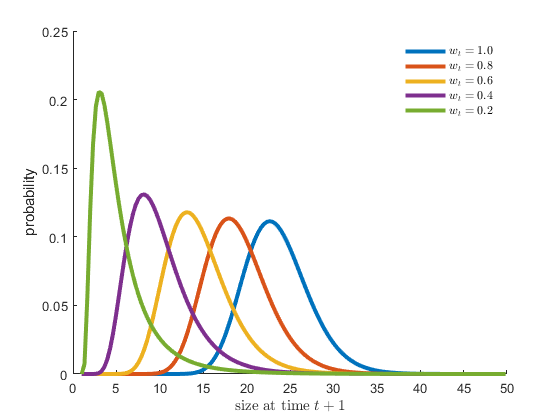
\includegraphics[width=0.7\linewidth]{Images/nonlinear_comparison}
	\caption{Plots of $g(y, x, w_t)$ for $x = 1$ and various values of $w_t$}
	\label{fig:nonlinear_comparison}
\end{figure}

Since smaller values of $w_t$ correspond to higher biomass, this plot indicates that a size $x=1$ individual is likely to grow less when total population biomass is high. The value $x=1$ is not special; other values of $x$ yield similar plots.

\begin{figure}
	
\end{figure}

\section{Simulation Results}

In the following subsections, we give simulation results based on the system \eqref{eqn:ipmsystem}, but with some caveats. We used MATLAB to generate a matrix at each time step which sampled the kernel of $T_{w_t}$ using a mesh of 300 equally spaced points on the $x-$ and $y-$axes; however, Corollary \ref{th:corollarytonotweaklycompact} says that $T_{w_t}$ is not compact for any value of $w_t \in (0,1]$, and hence cannot be approximated by matrices. Because of this, we do not claim that our simulations reflect the true dynamics of the infinite-dimensional system. Instead, one could think of the nonlinear IPM as a tool to generate a finite-dimensional system with as many size classes as mesh points as one chooses, and which allows for more growth options than the matrix $A_{w_t}$ in \cite{Callahan2019}.

With that said, we make one more assumption on the IPM model in three of the following subsections, namely that individuals all have the same survival rate, regardless of size. This is consistent with our assumption in Section \ref{section:operatordef}, in which we assumed $s(x)$ was increasing, but not necessarily strictly increasing. For constant survival, the simulations suggest that a result akin to Theorem \ref{thm:finitedimtheorem} may hold for the nonlinear IPM system. In subsections \ref{subsec:0.05f(x)}, \ref{subsec:f(x)}, and \ref{subsec:1000f(x)}, we assume that the survival probability for all sizes is $0.68$, which is the maximum survival rate given in \cite{Vindenes2014}. 

We decided to assume constant survival because the long-term behavior of the IPM system \eqref{eqn:ipmsystem} is unclear for the sigmoid-shaped survival function $s(x)$ given in \cite{Vindenes2014}. In this case, the survival of offspring is extremely low, and the resulting populations grow very slowly. Hence, it is hard to tell from plots what the population is doing in the long-run. With this more realistic survival function, the asymptotic behavior of the system is not at all clear, even after thousands of time steps. Hence, for this preliminary investigation, we will keep the survival rates for each size constant.

In the results that follow, we allowed the IPM system to evolve for 200 time steps, starting from five different initial populations $p_i = v_i/||v_1||_1$, where
\begin{align}
	v_i(x) = \begin{cases} 1, & x \in \left[L + \frac{1}{5}(U-L)(i-1), L + \frac{1}{5}(U-L)i \right] \\ 0, & \text{else} \end{cases}
\end{align}
for $i = 1, 2, 3, 4, 5$, and where $L$, $U$ are the lower- and upper-limits of $x$, respectively. These vectors give a different initial concentrations in ranges that span the whole state space $[L, U]$. Note also that $||p_i||_1 = 1$ for all $i$; we tested larger initial populations (up to 10,000 individuals), but changing the population size did not change the asymptotic behavior of the model.

In subsections \ref{subsec:0.05f(x)} - \ref{subsec:1000f(x)}, we investigated whether results like parts (2)-(4) of Theorem \ref{thm:finitedimtheorem} held. In the first simulations, we scaled the fecundity function $f(x)$ given in \cite{Vindenes2014} by 0.05, and in this case the population went extinct. Second, we left $f(x)$ unchanged, and this yielded a positive steady state population. Third, we scaled $f(x)$ by  a factor of 1000, which yielded a population going to infinity. In the respective simulations, the biomass went 0, a positive value $B^*$, and infinity. Hence, the operators $T_{w_t}$ appear to approach the linear operators $T_1$, $T_{w^*}$, or $T_{0.001}$, respectively, where
\[w^*:= \max \left\{ \frac{1}{1 + c B^*}, 0.001 \right\}.\]
Because of this, each of the normalized population vectors $p_t/||p_t||$ in Subsections \ref{subsec:0.05f(x)} - \ref{subsec:1000f(x)} approached a steady state distribution given by the leading eigenvector of the respective linear operators $T_1$, $_{w^*}$, and $T_{0.001}$. By only altering the fecundity function of the various kernels, we were able to directly compare these steady state distributions; this is because the different scaling factors on $f(x)$ disappear during  normalization, a fact guaranteed by the formula 
\[\psi = F(\lambda I - GS)^{-1}b\]
for the leading eigenvector of a the linear IPM operator (see Corollary \ref{th:existenceofevector}). Since this nonlinear IPM is a model of density-dependent somatic growth, directly comparing the steady state distributions allows us to verify that higher biomass leads to populations dominated by smaller individuals.

Before we give simulation results, we stress again that we do not know whether they accurately portray the dynamics of the infinite-dimensional system \ref{eqn:ipmsystem}. This is because for a fixed $w_t = w$, we cannot uniformly approximate the linear operator $T_w$ with matrices, since $T_w$ is not compact (see Theorem \ref{th:corollarytonotweaklycompact}. And if we cannot uniformly approximate a particular $T_{w}$, we also cannot make a claim about the asymptotic behavior of the full nonlinear system $\varphi_{t+1} = T_{w_t} \varphi_t$. Instead, we consider the following results to be for a high-dimensional matrix model, obtained by sampling the kernel \eqref{eqn:ddkernel} with $300^2$ mesh points. 

We summarize the functions and parameters we used in the following table:

\begin{table}[h!]
	\begin{center}
		\caption{Kernel functions and parameters}
		\label{tab:funcsandparams}
		\begin{tabular}{c|c|c}
			\hline
			 & \textbf{Description} & \textbf{Source}\\
			\hline \hline
			$b(y)$ & offspring distribution & \cite{Vindenes2014} \\
			$f(x)$ & fecundity & \cite{Vindenes2014} \\
			$g(y, x, 1)$ & somatic growth, no biomass & \cite{Vindenes2014} \\
			$s(x) \equiv 0.68$ & survival probability & \cite{Vindenes2014} \\
			$\alpha = 6.648 \times 10^{-6} \text{kg}/\text{cm}^3$ & conversion rate in \eqref{eqn:ipmbiomass} & \cite{Milardi2014} \\
			$\beta = 3.0217$ & power in \eqref{eqn:ipmbiomass} & \cite{Milardi2014} \\
			$c = 9.0 \times 10^{-3} \text{kg}^{-1}$ & factor in \eqref{eqn:wdef} & \cite{Chizinski2010}, converted to $\text{kg}^{-1}$ \\
			\hline
		\end{tabular}
	\end{center}
\end{table}

We note that the the papers \cite{Vindenes2014} and \cite{Milardi2014} both studied populations of northern pike (\emph{Esox lucius}), but \cite{Chizinski2010} modeled white perch (\emph{Morone americana}). We were unable to find a parameter $c$ in the literature for northern pike, so we tested values of $c$ on the order of $10^{-2}$ to $10^{-4}$, and found that the qualitative results of the simulations still held true.

\subsection{Simulations for the Fecundity Function $0.05f(x)$} \label{subsec:0.05f(x)}

In this subsection, we consider the IPM with fecundity function given by $0.05f(x)$. Recall that $w_t = 1$ corresponds is the limiting case corresponding to no biomass, i.e., when the population size is zero. Notwithstanding the fact that there are no individuals to do any growing, we expect this limiting case to be the ``best case" for growth, meaning we expect $r(T_w) < r(T_1)$ for any $w<1$. Hence, we also expect the population to die out if $r(T_1)<1$. In the case of the matrix model in \cite{Callahan2019}, this is the second conclusion of Theorem \ref{thm:finitedimtheorem}.

Using the $\eig()$ function in MATLAB, we estimated that $r(T_1) \approx 0.984 < 1$, and Figure \ref{fig:spectralradiuswhenf=0.05} suggests that $r(T_{w_t}) \to r_(T_1)$ for the initial populations $\varphi_0 = p_i$:

\begin{figure}[H]
	\centering
	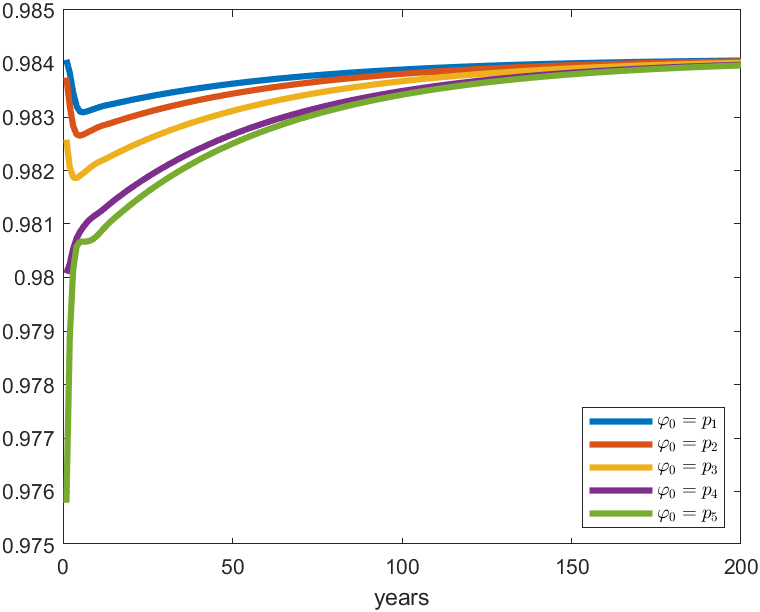
\includegraphics[width=0.7\linewidth]{Images/F=0.05/spectral_radius_when_f=0.05}
	\caption{Spectral radius of $T_{w_t}$ when fecundity is $0.05f(x)$}
	\label{fig:spectralradiuswhenf=0.05}
\end{figure}

Since the spectral radii $r(T_{w_t})$ appear to converge to the value $r(T_1)$, where the latter is the growth rate when the biomass is zero, one may wonder if the total population and biomass in fact go to zero. This does appear to be the case:

\begin{figure}[H]
	\centering
	\begin{minipage}{.48\textwidth}
	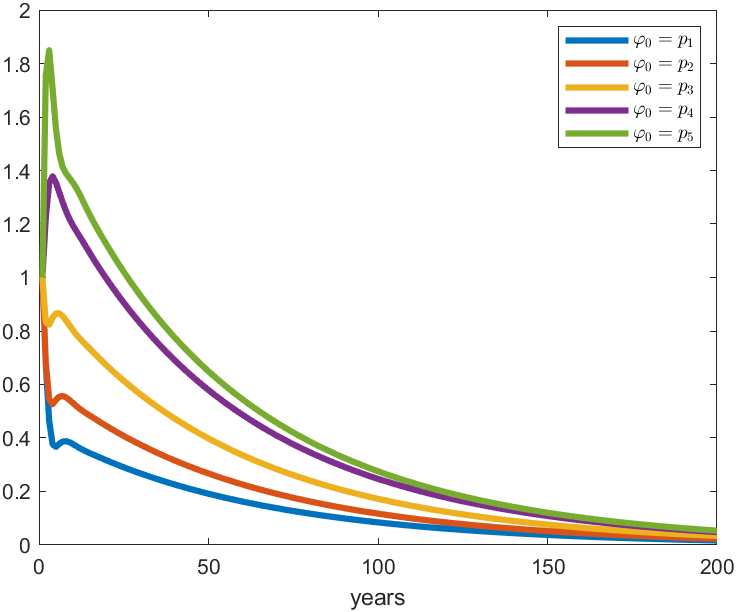
\includegraphics[width=\linewidth]{Images/F=0.05/total_pop_when_f=0.05}
	\caption{Total population}
	\label{fig:totalpopwhenf=0.05}
	\end{minipage} \quad 
	\centering
	\begin{minipage}{.48\textwidth}
	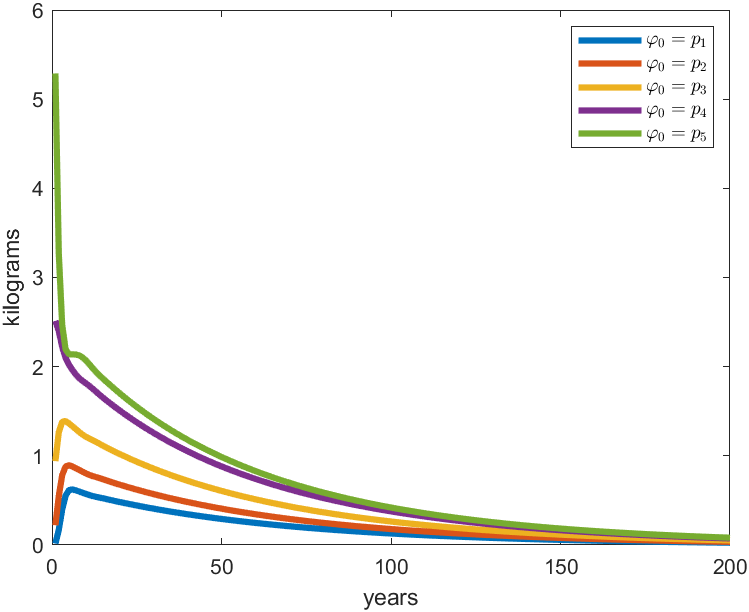
\includegraphics[width=\linewidth]{Images/F=0.05/total_biomass_when_f=0.05}
	\caption{Total biomass}
	\label{fig:totalbiomasswhenf=0.05}
	\end{minipage}
\end{figure}

Even though the population vectors $\varphi_t$ approach 0, the normalized vectors $\varphi_t / || \varphi_t||$ converge to a stable stage distribution, which is the leading eigenvector of $T_1$. Note that $T_1$ is the same as the linear operator with kernel \ref{eqn:kernel}, which incorporates no density-dependence in somatic growth. Hence, this is the distribution we compare later distributions with in order to determine whether a population is dominated by small individuals:

\begin{figure}[H]
	\centering
	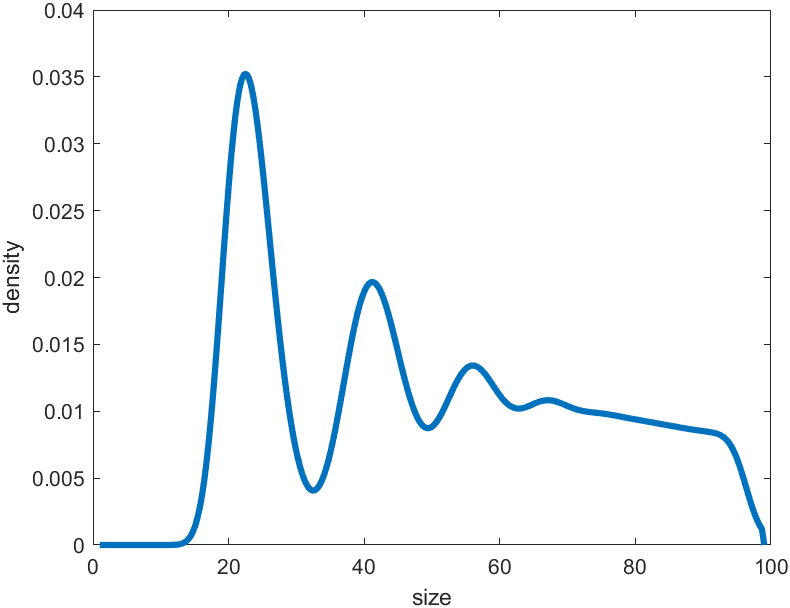
\includegraphics[width=0.7\linewidth]{Images/F=0.05/ssd_when_f=0.05}
	\caption{Stable stage distribution, also the leading eigenvector of $T_1$}
	\label{fig:ssdwhenf=0.05}
\end{figure}

Note that the sharp decrease near the upper size limit $U$ is a result of the difficulty in approximating the kernel near $(U,U)$, since the kernel is unbounded in any neighborhood of that point.

\subsection{Simulations for the Fecundity Function $f(x)$} \label{subsec:f(x)}

For the kernel with fecundity function $f(x)$, we found that $r(T_{0.001}) < 1 < r(T_1)$, a situation similar to conclusion (4) of Theorem \ref{thm:finitedimtheorem}. That result states that the matrix system \eqref{eqn:system} approaches a nonzero equilibrium population. In other words, $r(A_{w_t}) \to 1$, which also appears to happen in the case of the IPM system:

\begin{figure}[H]
	\centering
	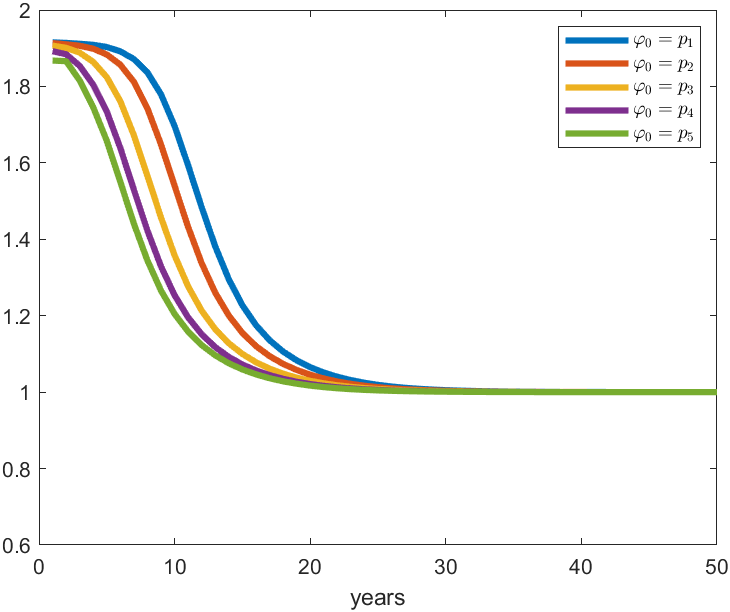
\includegraphics[width=0.7\linewidth]{Images/F=1/spectral_radius_when_f=1}
	\caption{Spectral radius of $T_{w_t}$ when fecundity is $f(x)$}
	\label{fig:spectralradiuswhenf=1}
\end{figure}

Additionally, the total population and biomass approach positive values:

\begin{figure}[H]
	\centering
	\begin{minipage}{.48\textwidth}
		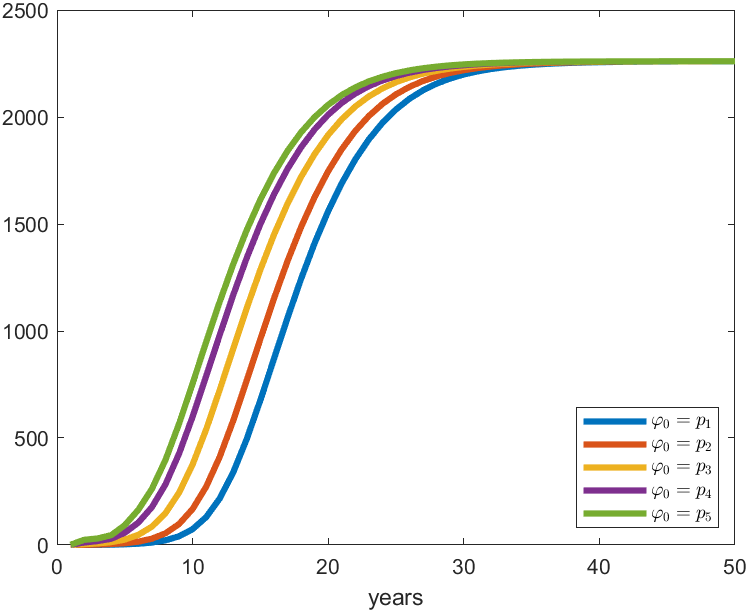
\includegraphics[width=\linewidth]{Images/F=1/total_pop_when_f=1}
		\caption{Total population}
		\label{fig:totalpopwhenf=1}
	\end{minipage} \quad 
	\centering
	\begin{minipage}{.48\textwidth}
		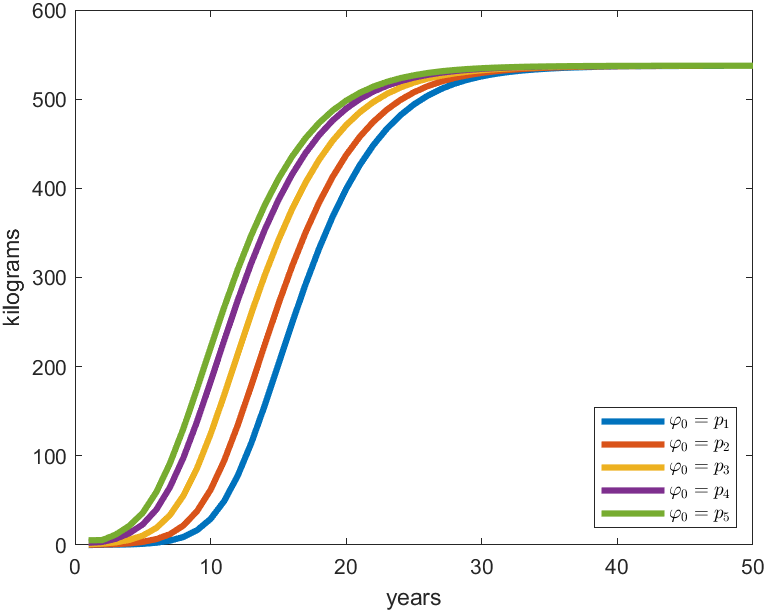
\includegraphics[width=\linewidth]{Images/F=1/total_biomass_when_f=1}
		\caption{Total biomass}
		\label{fig:totalbiomasswhenf=1}
	\end{minipage}
\end{figure}

In this case, the population vector converges to an equilibrium distribution, which is also the leading eigenvector of $T_{w(B^*)}$, where $B^*$ is the equilibrium biomass indicated in Figure \ref{fig:totalbiomasswhenf=1}:

\begin{figure}[H]
	\centering
	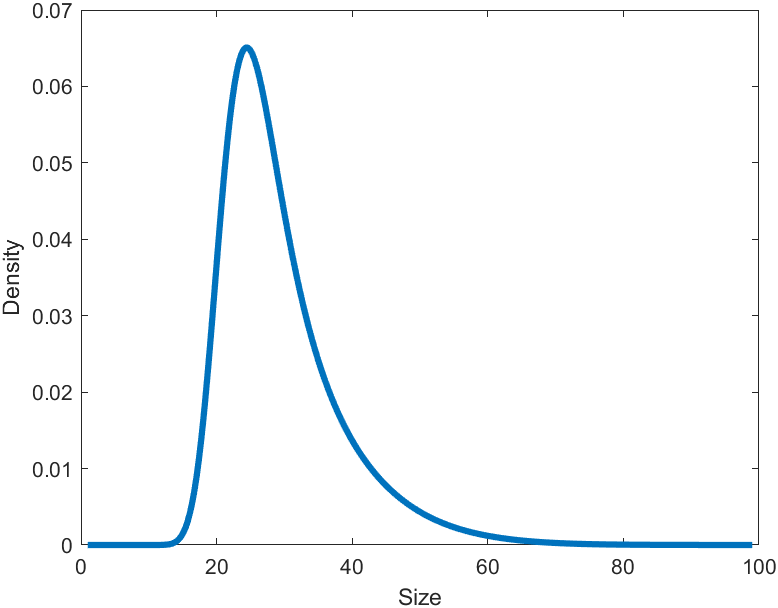
\includegraphics[width=0.7\linewidth]{Images/F=1/ssd_when_f=1}
	\caption{Stable stage distribution, also the leading eigenvector of $T_{w(B^*)}$}
	\label{fig:ssdwhenf=1}
\end{figure}

Note the contrast between Figures \ref{fig:ssdwhenf=0.05} and \ref{fig:ssdwhenf=1}; when the total biomass approaches a positive value, the stable stage distribution shows inhibited growth. The distribution in Figure \ref{fig:ssdwhenf=1} is more concentrated in small sizes, and individuals do not grow much past the spike of the offspring distribution.

\subsection{Simluations for the Fecundity Function $1000f(x)$} \label{subsec:1000f(x)}

Conclusion (3) of Theorem \ref{thm:finitedimtheorem} gives a sufficient condition for the population to grow without bound, namely when $r(A_0) >1$. In order to avoid division by zero in our model, the lowest value $w_t$ can attain is $0.001$, so we investigated whether the population in the IPM model goes to infinity when $r(T_{0.001}) > 1$. This occurs for a fecundity function given by $1000f(x)$, but even with this dramatic increase, our estimate for $r(T_{0.001})$ was only barely greater than 1. In this case, we expected $r(T_{w_t}) \to r(T_{0.001}) > 1$, which does appear to be the case. In the following plot, we included a dotted line to show that the spectral radii stay bounded away from (and above) 1:

\begin{figure}[H]
	\centering
	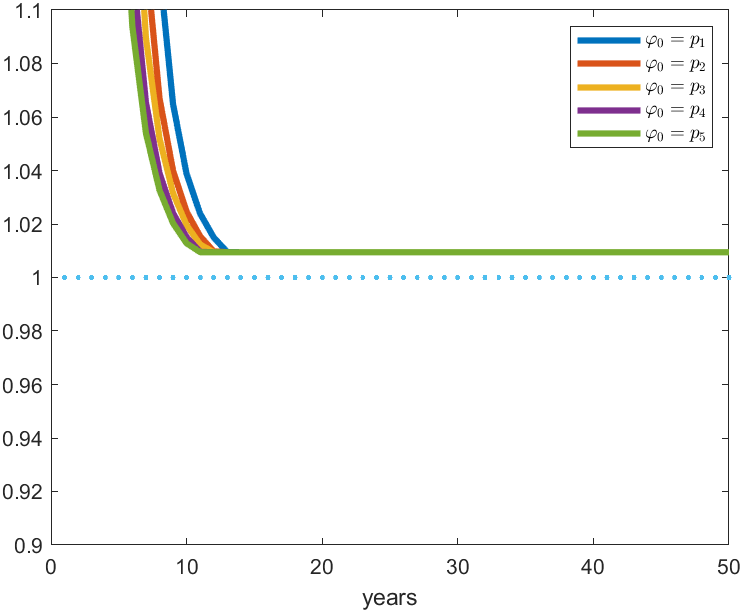
\includegraphics[width=0.7\linewidth]{Images/F=1000/spectral_radius_when_f=1000}
	\caption{Spectral radius of $T_{w_t}$ when fecundity is $1000f(x)$}
	\label{fig:spectralradiuswhenf=1000}
\end{figure}

As expected, the total population and biomass increase without bound:

\begin{figure}[H]
	\centering
	\begin{minipage}{.48\textwidth}
		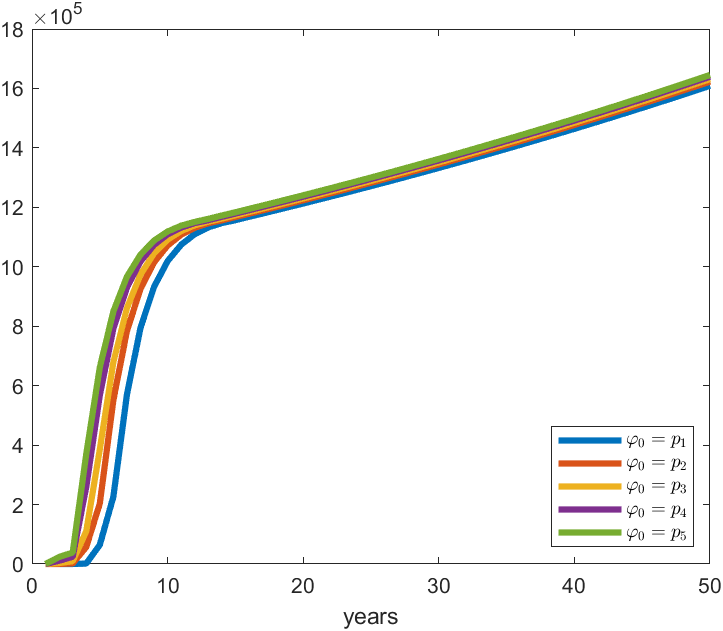
\includegraphics[width=\linewidth]{Images/F=1000/total_pop_when_f=1000}
		\caption{Total population}
		\label{fig:totalpopwhenf=1000}
	\end{minipage} \quad 
	\centering
	\begin{minipage}{.48\textwidth}
		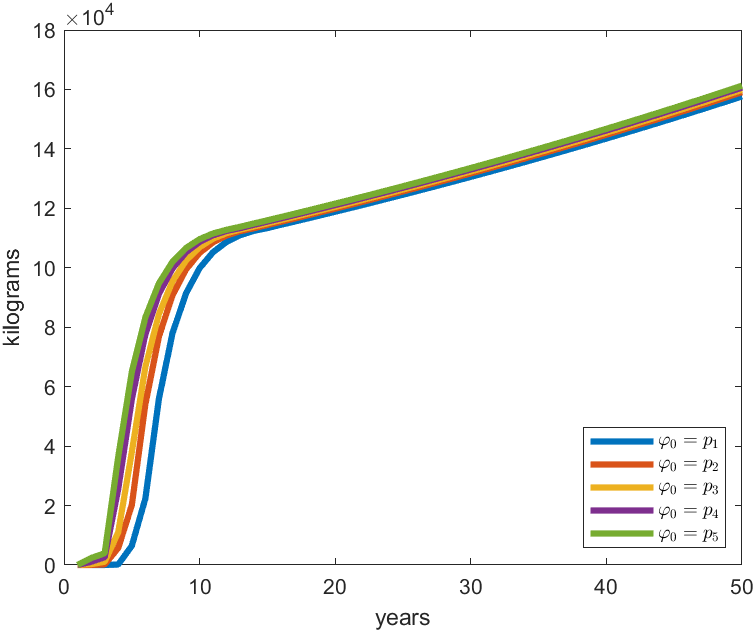
\includegraphics[width=\linewidth]{Images/F=1000/total_biomass_when_f=1000}
		\caption{Total biomass}
		\label{fig:totalbiomasswhenf=1000}
	\end{minipage}
\end{figure}

Since the biomass increases without bound, the values $w_t$ eventually attain the lower bound $0.001$, and the population increases at a rate given by $r(T_{0.001})$. Hence, the population growth is eventually modeled by a linear function, and the stable stage distribution is the leading eigenvector of $T_{0.001}$:

\begin{figure}[H]
	\centering
	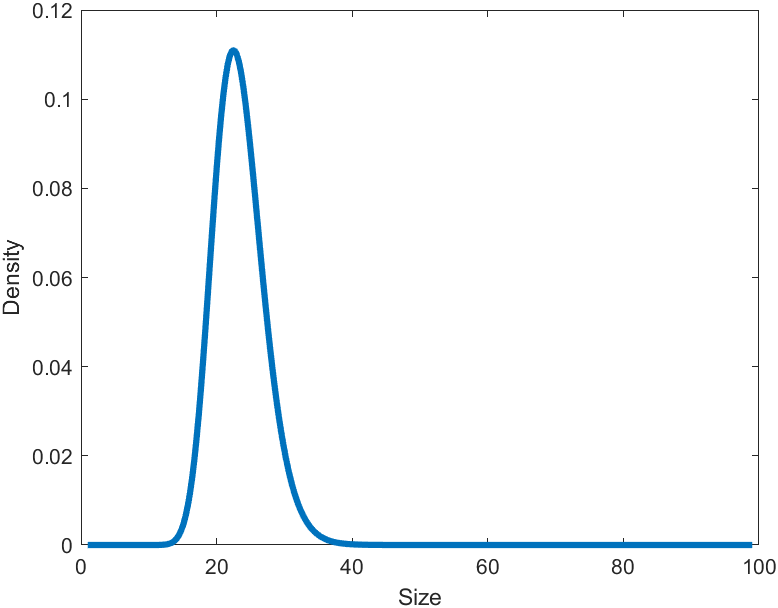
\includegraphics[width=0.7\linewidth]{Images/F=1000/ssd_when_f=1000}
	\caption{Stable stage distribution}
	\label{fig:ssdwhenf=1000}
\end{figure}

Note that Figure \ref{fig:ssdwhenf=1000} indicates a more extreme case of inhibited growth than in Figure \ref{fig:ssdwhenf=1}, since the biomass continues to increase (though $w_t$ attains its lower bound of 0.001).















%% backmatter is needed at the end of the main body of your thesis to
%% set up page numbering correctly for the remainder of the thesis
\backmatter

%% Start the correct formatting for the appendices
%\appendix
%%% Input each appendix here
%\input{./appendix_a}

% \bibliographystyle{alpha}  % or use  abbrv to abbreviate first names and use numerical indices
\bibliographystyle{abbrv}  % or use  abbrv to abbreviate first names and use numerical indices
%% Add your BibTex file here (don't include the .bib)
\bibliography{references}

\end{document}

\endinput
